\documentclass[a4paper,12pt]{report}
\usepackage[utf8]{inputenc}
\usepackage[magyar]{babel}
\usepackage{indentfirst}
\usepackage{textcomp}
\usepackage{listings}
\usepackage{graphicx}
\usepackage{epstopdf}
\usepackage[inner=3.5cm,outer=2.5cm,top=2.5cm, bottom=2.5cm]{geometry}
\RequirePackage{geometry}
\geometry{inner=3.5cm,outer=2.5cm,top=2.5cm, bottom=2.5cm} \linespread{1.3}
\lstset{language=C++, basicstyle=\ttfamily, breaklines=true}
\widowpenalty=30000
\clubpenalty=30000
\frenchspacing
\sloppy

\usepackage{etoolbox,refcount}
\usepackage{multicol}

\newcounter{countitems}
\newcounter{nextitemizecount}
\newcommand{\setupcountitems}{%
  \stepcounter{nextitemizecount}%
  \setcounter{countitems}{0}%
  \preto\item{\stepcounter{countitems}}%
}
\makeatletter
\newcommand{\computecountitems}{%
  \edef\@currentlabel{\number\c@countitems}%
  \label{countitems@\number\numexpr\value{nextitemizecount}-1\relax}%
}
\newcommand{\nextitemizecount}{%
  \getrefnumber{countitems@\number\c@nextitemizecount}%
}
\newcommand{\previtemizecount}{%
  \getrefnumber{countitems@\number\numexpr\value{nextitemizecount}-1\relax}%
}
\makeatother    
\newenvironment{AutoMultiColItemize}{%
\ifnumcomp{\nextitemizecount}{>}{3}{\begin{multicols}{2}}{}%
\setupcountitems\begin{itemize}}%
{\end{itemize}%
\unskip\computecountitems\ifnumcomp{\previtemizecount}{>}{3}{\end{multicols}}{}}

\renewcommand{\lstlistingname}{Kódrészlet}% Listing -> Algorithm
\renewcommand{\lstlistlistingname}{\lstlistingname ek}% List of Listings -> List of Algorithms


\title{Statikus elemzések tervezése \emph{Clang} eszközzel}
\author{Fülöp Endre}
\begin{document}

\input titlepage

\tableofcontents

\chapter*{Köszönetnyilvánítás}
Köszönettel tartozom a témavezetőmnek, Pataki Norbernek, aki lelkiismeretes munkájával felügyelte a dolgozat tartalmi és formai alakulását. Köszönöm a lehetőséget az Ericsson csapatának, többek között Krupp Dánielnek, Horváth Gábornak és Gera Zoltánnak, a velük töltött munka inspiráló volt számomra. Nem utolsó sorban köszönöm a családomnak, hogy türelemmel viseltettek irányomban a tanulmányaim és a dolgozat írása alatt.

\chapter{Bevezetés}
\section{Motiváció}
A szoftverkörnyezetek nagyon változatosak, és mindnek megvannak a megoldandó problémái, illetve az ezek megoldásához természetesen illeszkedő programozási nyelvek. Ebből fakadóan a fejlesztési és futási követelmények, illetve az ezeket támogató módszerek tekintetében is nagy eltérések tapasztalhatóak.

A szoftverfejlesztés során egy, a specifikációban körvonalazott problémára keressük a megoldást valamilyen információs rendszer megfelelő megtervezésével és megvalósításával. A problémához illeszkedő elvi megoldás megtalálása csak egy korai lépés a teljes folyamatot tekintve. Az ezt követő megvalósítás során pedig jellemzően a kiválasztott programozási nyelven implementálásra kerülnek a megoldás algoritmusai. Ez a lépés már magában nagy többletkomplexitást adhat sok projekthez. Ennek okai többek között lehetnek:
\begin{itemize}
\item modularizálás az újrafelhasználhatóság növelése érdekében
\item a megfelelő külső könyvtárak elérhetővé tétele és verziókezelése
\item egyéb elő- és utófeldolgozást végző rendszerek
\begin{itemize}
\item fordítás és forrástranszformáció
\item csomagolás, függőségek feloldása
\item kihelyezés, eljuttatás a futási környezetbe (deployment)
\end{itemize}
\end{itemize}
Ilyen körülmények között érdemes lehet automatizált eszközöket bevetni annak biztosítására, hogy a szoftver helyes működését ellenőrizni tudjuk.

Szakdolgozatomban egy speciális, potenciálisan hasznos eredményeket produkáló szeletét vizsgálom az említett eszköztárnak, a tesztelési fázis során futó, szoftverhelyességet vizsgáló hibakereső eszközöket. Ezen belül bemutatom a fordításidőben történő hibakeresés jelenleg egyik legfejlettebb eszközét, a statikus analízist, és egy példaprogramon belül demonstrálom a lehetőségeit, illetve \emph{Clang} eszközzel való implementáció részleteit.

A szakdolgozat a C nyelvcsaládbeli példák alapján mutatja be a statikus analízist, a megvalósított ellenőrző program is C illetve C++ nyelveken végez ellenőrzést, illetve a \emph{Clang} is egy C++-ban megvalósított projekt. Emellett azonban sok más, akár teljesen más paradigmákat képviselő programozás nyelv forráskódelemzése is aktívan vizsgált téma, és a bemutatott elvek közül sok érvényes ezekre is. Általánosan elmondható, hogy minél több a közös pont a kérdéses programnyelv és az erősen típusos, fordított, és hardverközeli C++ nyelv között, a szakdolgozat annál nagyobb része szolgálhat releváns információval.

\section{Hibakeresés}
A szoftverfejlesztés implementációs fázisát sok esetben egy tesztelési eljárás követi. Ennek célja, hogy megbizonyosodjunk arról, hogy a specifikációban leírt működést produkálja a szoftver, illetve esetleg más esztétikai és kényelmi feltételeket teljesít-e.
A tesztelés a program élettartamának számos pontján hatékonynak bizonyulhat. A hibakeresés lehetséges:
\begin{itemize}
\item tervezési fázisban, egy még absztrakt programleíró modellen
\item megvalósítás közben, az implementációs programnyelven
\item implementáció után, a fordítást követő reprezentáción, ez lehet:
\begin{itemize}
\item bytekód
\item tárgykód
\item köztes reprezentáció
\end{itemize}
\item futtatás előtt (pl. unit tesztek), futásidejű tesztekkel (pl. integrációs és performancia tesztek)
\item rendeltetésszerű használat során a futási környezetben \cite{chaosmonkey}
\end{itemize}

\subsection{Absztrakt hibakeresés}
A szoftvertervezés korai szakaszában gyakran elvont ábrázolási módszereket vetnek be, mint például UML diagramok. Sokféle szerepet elláthatnak, például osztálydiagramok segítségével írják le a program strukturális szerkezetét, felhasználói-eset diagram segítségével a felhasználói interakciókat, szekvencia-diagramok segítségével pedig a programfolyamatok egymáshoz képesti ok-okozati, időbeli viszonyát. Már egy ilyen korai fázisban is érdemes lehet vizsgálni a szoftvert, a szekvenciadiagramok validáció és verifikáció módszerét használó elemzése  \cite{umlverification} már fejlesztői környezeteken belül is elérhető, a fejlesztési folyamat szerves részévé válhat.

\subsection{Forráselemzés}
Sok programozási nyelv esetében a forráskódot nem közvetlenül értelmezi a futtató környezet, hanem egy transzformációs lépésen át kell haladnia. A fordítás során jellemzően emberi feldolgozásra alkalmas formából valamilyen gépi szinten könnyebben értelmezhető alakba jutunk. Hogy ilyen előfeldolgozást használ sok nyelv, annak többek között a program teljesítményéhez van köze. A C++ esetében például kifejezetten sok eszköz áll rendelkezésre, hogy azokat az információkat, amelyek a kód írása során rendelkezésre állnak, hatékonyan fel lehessen használni. A template metaprogramming technika például a C++ esetében egy teljes értékű programozási nyelvet alkot, melynek segítségével sok problémát már fordításidőben meg lehet oldani, illetve csökkenteni lehet a program futásidejét a fordításra szánt idő rovására.
Jellemzően a fordítást megelőzően egy ellenőrző lépés keretében történik a vizsgálat, vannak azonban csak értelmezett (interpretált) nyelvek is. Ezek esetében is meg lehet vizsgálni a forráskódot, és az alapján is lehet érvelni a majd futó program tulajdonságait illetően.

Szakdolgozatomban a forráselemzés kitüntetett szerepet kap, a statikus analízis a forráselemzés jelenleg legnagyobb komplexitással bíró eleme, mind a detektálásra szánt idő, mind a felismerhető problémák körét tekintve. Azonban a forráselemzés más technikákat is magába foglal. Forráselemzéshez a program forráskódjának minden lehetséges szinten történő elemzése:
\begin{itemize}
\item lexikális, vagyis, hogy a program megengedett tokenek sorozatából áll
\item szintaktikai, mely során megvizsgáljuk, hogy a tokensorozat megengedett nyelvi elemeket ír le
\item szemantikai, a program jelentésével foglalkozó elemzés, vagyis hogy a program által leírt működés valóban megoldja-e a kitűzött problémát
\end{itemize}
A forráselemzés jobb kifejezés, mint a fordításidejű analízis, mert interpretált nyelvek esetében is van értelme a forrást vizsgálni. A módszerek, melyek a forráskódot mint olyan reprezentáció vizsgálják, amelyen automatizált elemzéseket és transzformációkat \cite{interpretedtransforms} lehet végrehajtani, egyre elterjedtebbek. A transzformációk célja lehet lehet többek között optimalizáció, vagy a futtatási környezethez való alkalmazkodás.

Erre példa lehet a javascript programozási nyelv, mely egy alapvetően interpretált, böngészőszoftverekben elterjedt nyelv. A nyelvi sztenderd fejlődése gyors a böngészők támogatásának elterjedéséhez képest, illetve régebbi böngészőverziók nem támogatnak bizonyos újabb nyelvi elemeket. Ennek köszönhetően az új sztenderd szerint helyes kódbázis nem kompatibilis a régi böngészőkkel. Ezt a problémát egy forrástranszformációs technikával \cite{transpilation} oldják meg, mely során az új nyelvi elemeket forráskód szintjén lecserélik egy olyan implementációra, mely viselkedését tekintve megegyezik az újjal, és kompatibilis a régi sztenderddel is.

\subsubsection{Szintaktikai elemzés}
Fordított programnyelvek esetében egyértelmű követelmény, hogy a forráskód minden részének helyesnek kell lennie a nyelv szabályai szerint, különben már a fordító hibaüzenettel jelez. Jó lehetőséget ad azonban ez a módszer nem fordított nyelveknél is, ahol ha ezeket az elemzéseket előre el tudjuk végezni az egész kódbázison, akkor sok hibát kiszűrhetünk.
\subsubsection{Egyszerű szemantikai elemzés}
Egyszerű szemantikai elemzés esetében a forráskód alapján döntéseket hozunk a program jelentésének, várható viselkedésének helyességéről. Tipikusan egyszerűbb, nyilvánvalóan helytelen, illetve teljesen felesleges utasítok szűrhetőek ki ilyen módon. Jellemző példa lehet egy változó önértékadása, amely legtöbb esetben egy üres-művelet és a fejlesztő figyelmetlenségéből ered.
Példa C++ esetében, tegyük fel, hogy egy közönséges függvény törzsében vagyunk:
\begin{lstlisting}
int a = 0;
a = a;
\end{lstlisting}
\subsubsection{Összetett szemantikai elemzés}
Látható, hogy ha a fenti példában nem szerepelne a változó nullára inicializálása sem, akkor még egy problémával találkoznánk: inicializálatlan változó értékének használata. Ennek a problémának a felderítése azonban általános esetben sokkal nehezebb, mint egy közönséges önértékadás felfedezése. Szükség van arra, hogy a programozási nyelv szabályait követve meghatározzuk azt a környezetet, ahol a használatot megelőzően potenciálisan értéket kaphatott a változó, majd fel kell deríteni, hogy ez tényleg megtörtént-e.
\begin{lstlisting}[caption={Szemantikailag hibás függvény}\label{lst:noclosefunction},language=C]
void simple_read(char *file, char *dst, size_t size) {
  int fd = open(filename, 0);
  read(fd, dst_buffer, buffer_size);
  // nincs close hivas
}
\end{lstlisting}
A fenti példa a UNIX rendszerek alapvető I/O műveleteivel olvas ki egy fájlból valamennyi bájtnyi adatot egy céltárolóba. A fenti függvény szintaktikailag helyes, és még ha hiányzik is belőle az \texttt{open} és a \texttt{read} függvények visszatérési értékének ellenőrzése, a legtöbb esetben az elvárt módon viselkedik. Mindenesetre addig, ameddig a folyamat el nem éri a számára megnyitható fájlleírók számát. Az \texttt{open} függvény ugyanis egy rendszerhívás köré írt vékony csomagoló, amely erőforrást foglal le a rendszerben. Az elvárt használata ennek az API-nak, hogy amikor végeztünk az erőforrás használatával, egy \texttt{close} hívással értesítsük erről a rendszert is. A rendszer felszabadítja az erőforrást, és a folyamat leírók lefoglalására szánt kerete visszaáll.
Az ilyen jellegű hibák felismerésére több információval kell rendelkeznünk a nyelv szintaktikai szabályainál, és a detektálás során is szükséges, hogy egy kódot alaposabban megvizsgáljuk. A fenti példában a hiba felismeréséhez szükség van a következő információkra:
\begin{itemize}
\item volt egy \texttt{open} hívás
\item az \texttt{open} hívás visszatérési értékével, mint paraméterrel nem volt hívás a \texttt{close} függvényre
\end{itemize}
Az, hogy egy változóban tároljuk el az \texttt{open} hívás értékét, technikai részlet. Mégis fontos, mert nem lenne sok értelme egy megnyitott leírót rögtön bezárni, és a hibakeresés lehetőségétől is elesnénk.
Valójában azt is mondhatjuk, hogy minden szemantikailag helyes használata ennek az API-nak feltételezi, hogy a fájlleíró értékét a memóriában őrizzük, ameddig ténylegesen használjuk az erőforrást. Mindezt azért, mert így később fel tudjuk szabadítani. Az eddigi észrevételeinket az alábbi módon egészíthetjük ki:
\begin{itemize}
\item volt egy \texttt{open} hívás
\item az \texttt{open} hívás visszatérési értékét egy változó formájában eltároljuk a memóriában, jelenleg ez az \emph{fd}
\item az \emph{fd} változó élettartamszabályai által meghatározott kódrészben sehol sem történt az \emph{fd} változóval paraméterezett \texttt{close} hívás
\end{itemize}
Ha ilyen formában fogalmazzuk meg a problémát, akkor elég ránézni a kódrészlethez tartozó szintaxisfára. Ezt és még sok, az analízist, és fejlesztést megkönnyítő funkciót a \emph{Clang} eszköz a rendelkezésünkre bocsát. A következő parancs segítségével szöveges formába ki tudjuk kérni a szöveges szintaxisfa-reprezentációt.
\begin{lstlisting}[caption={Az ast-dump használata}
\label{lst:astdump}]
clang --analyze -Xanalyzer -ast-dump file_read.c
\end{lstlisting}

\begin{figure}[h]
\centering
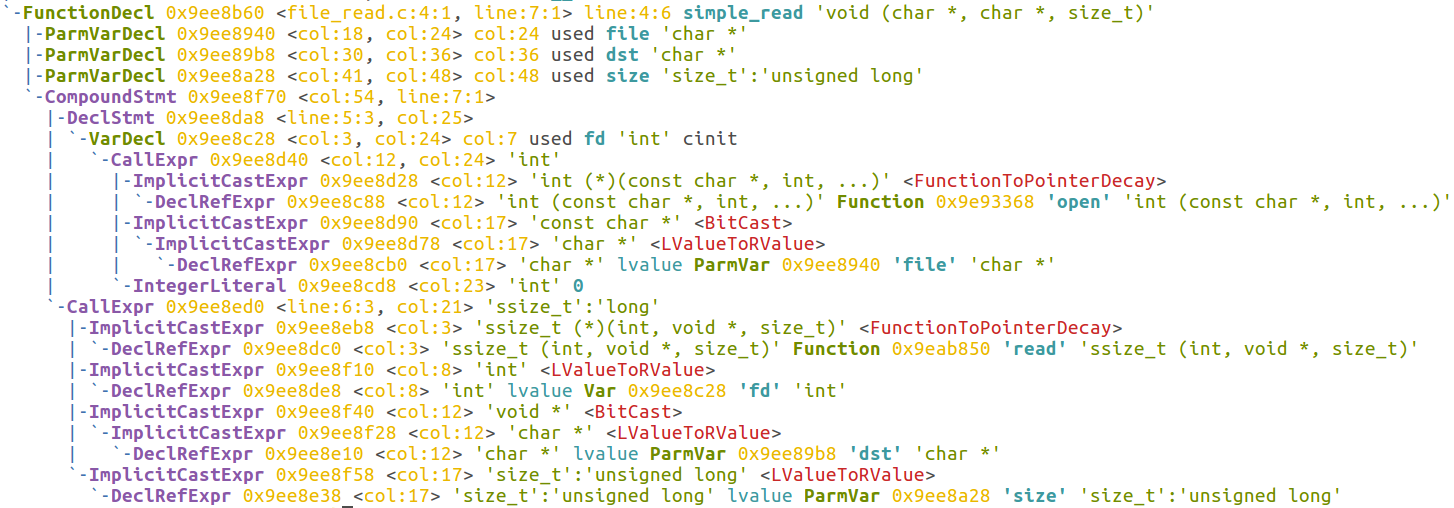
\includegraphics[scale=0.27]{astdumptomorrow.png}
\caption{Szintaxisfa szöveges megjelenítése.}
\end{figure}

Lehetőség van arra is, hogy a szintaxisfát grafikusan megjelenítsük, ezt a \emph{Clang} úgy támogatja, hogy egy \emph{dot} formátumú fájlt generál, amit platformspecifikusan meg lehet tekinteni valamilyen eszközzel, én az Ubuntu rendszeren elérhető xdot programot használtam.
\begin{lstlisting}[caption={Az ast-view használata}
\label{lst:astview}]
clang --analyze -Xanalyzer -ast-view file_read.c
\end{lstlisting}

\begin{figure}[h]
\caption{Szintaxisfa grafikus megjelenítése.}
\centering
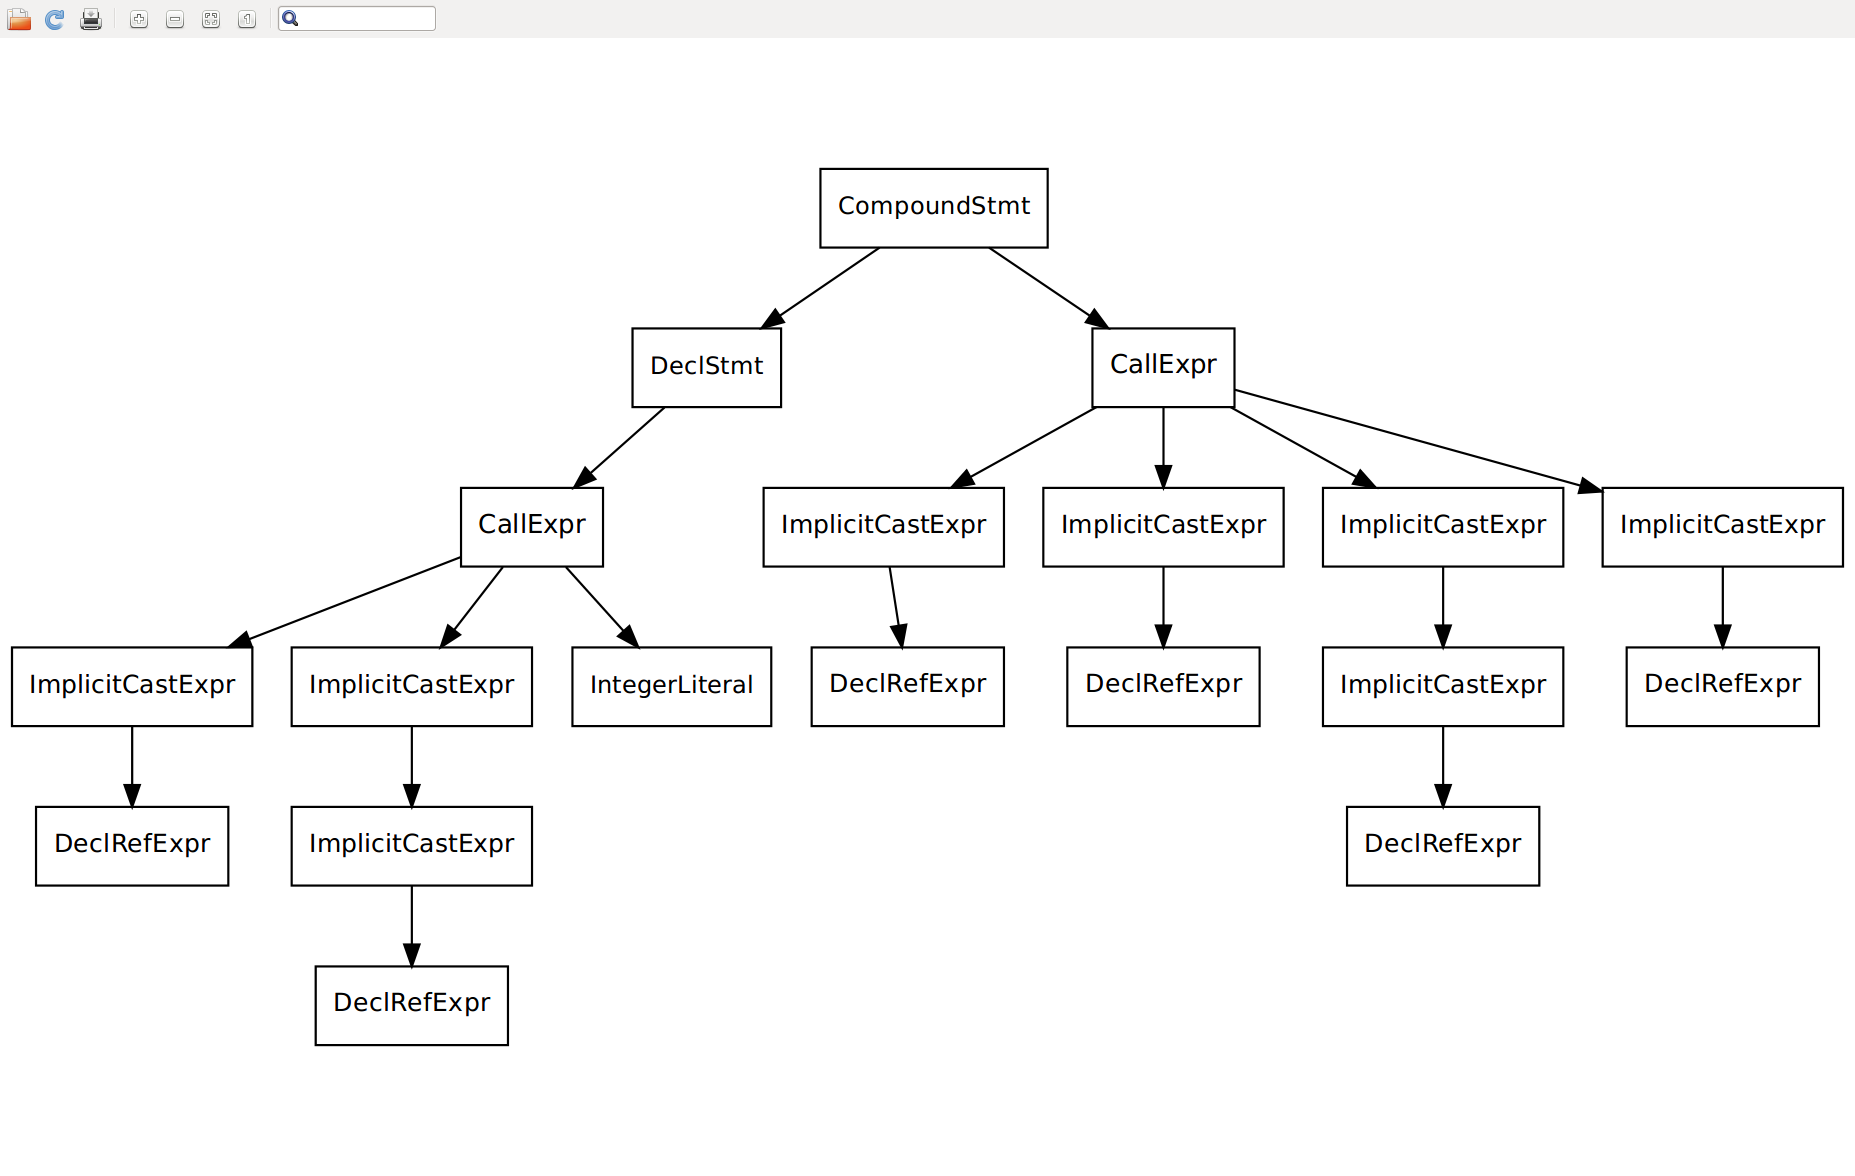
\includegraphics[scale=0.2]{astview.png}
\end{figure}

Látható, hogy a hiba feltárásához nem elég a szintaxisfa áttekintése, mégis az ilyen jellegű hibák felismeréséhez szükséges információ szerepel a benne. Szükség van a folyamat futásának modellezésére is, amelyet egy Control Flow Graph, vagy CFG segítségével tudunk szemléltetni (lásd ábra \ref{fig:facorialiterative}). Ilyen esetben fordulhatunk szimbolikus végrehajtás technikájához. A szimbolikus végrehajtás során szimuláljuk a program futását, azonban nem konkrét értékekkel, hanem az ezeket reprezentáló szimbolikus értékekkel. Az analízis során pedig az ezekre megfogalmazott kényszerek, és feltételek alapján tudunk következtetéseket levonni a kód helyességét illetően. A mai eszközök jellemzően a megszorításokról való érvelést visszavezetik egy SAT kielégíthetőségi problémára, amely során az aktuális programállapotban a változók lehetséges értékkészletét próbáljuk meg leszűkíteni. Ilyen módon ha kielégíthetetlen állapothoz értünk akkor már a nyelv szabályai segítségével tudunk érvelni a futási utak bejárhatóságágról is.

\begin{minipage}{\linewidth}
\begin{lstlisting}[caption={A faktoriális iteratív algoritmusa}
\label{lst:factorialiterative}]
unsigned factiter(unsigned n)
{
    unsigned accumulator = 1;
    if (n <= 1) return accumulator;
    while (n > 1)
    {
        accumulator *= n;
        n--;
    }
    return accumulator;
}
\end{lstlisting}
\end{minipage}

\begin{figure}[h]
\caption{Az iteratív faktoriális CFG-ja.}
\centering
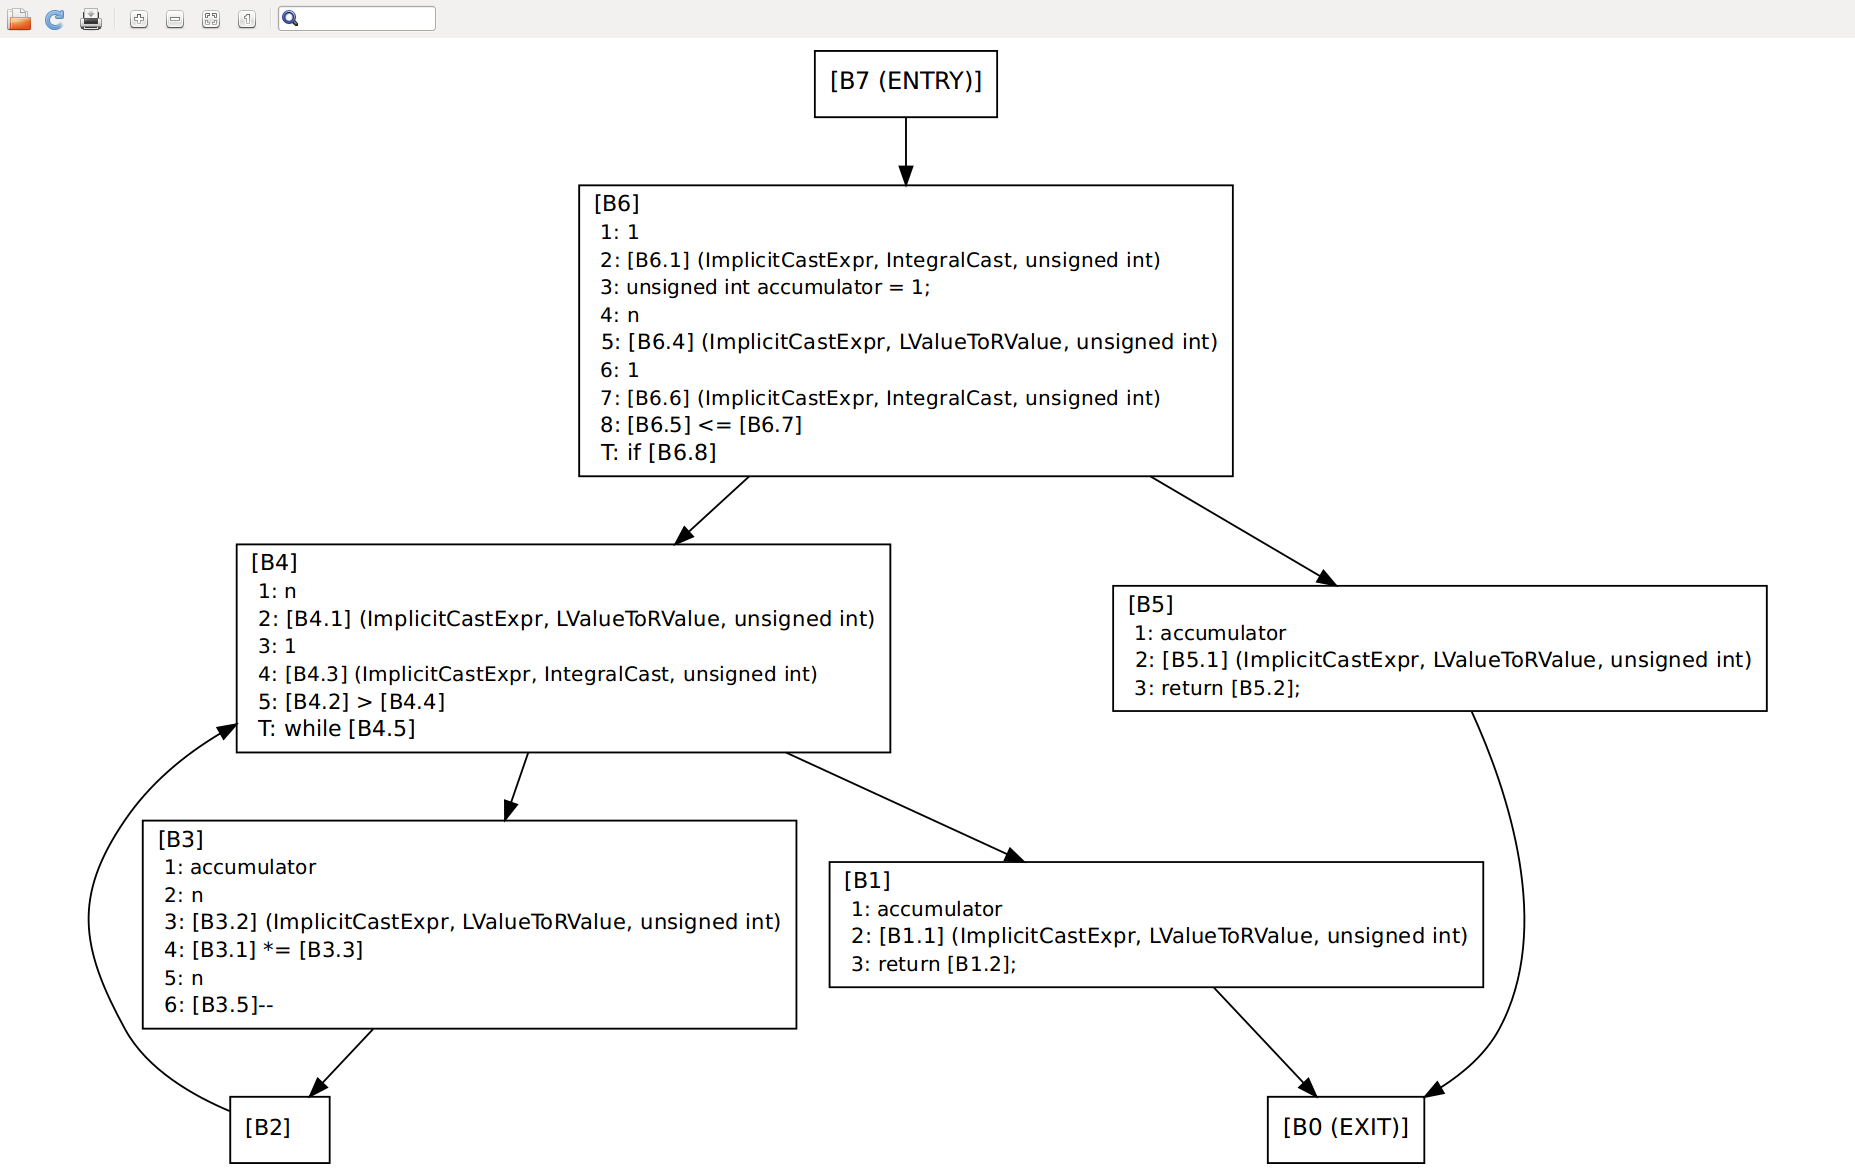
\includegraphics[scale=0.2]{factiter_cfg.png}
\label{fig:facorialiterative}
\end{figure}

\subsection{Futásidejű hibakeresés}
Kézenfekvő lehet a program működését menet közben megfigyelni. Ilyen esetben valamilyen eszköz segítségével az elkészült program futási tulajdonságait vizsgáljuk. Ezen eszközök is széles skálán mozoghatnak interaktivitás, hatókör és az éppen vizsgált program formáját tekintve.

A futásidejű hibakeresés más hibák felfedezésére képes, mint az előbbi módszerek. Bizonyos szempontból több hibát fel tud ismerni, hiszen futás közben több információ áll már rendelkezésünkre, hiszen program használata közben fogadott inputok ilyenkor kapnak konkrét értéket. Ez a többletinformáció biztossá teheti például egy, a szoftvervizsgálat korábbi szakaszaiban csak valószínűsíthető hiba tényleges fennállását, vagy teljesen új hibás működésekre is felhívhatja a figyelmet. Mindemellett hátrányokkal is rendelkezik az eddig megismert módszerekkel szemben. A futásidejű hibakeresés csak olyan hibákat tud felfedezni a programban, amelyhez tartozó kódrészletek ténylegesen használatra kerülnek futás során.

Tegyük fel például, hogy van egy szoftver, melyet programkönyvtárként akarunk felhasználni. Ekkor ha futásidejű hibakeresést akarunk végezni, akkor szükségünk van olyan kódokra, amely ezt a könyvtárt felhasználja. Az is szempont lehet, hogy minél nagyobb mértékben legyen egy könyvtár ilyen módon letesztelve, hiszen sok egymással csak érintőlegesen kapcsolódó részből is állhat egy programkönyvtár. Ennek mérésére bevezetésre került pár metrika is, melyek kódminőség szempontjából jellemzik a szoftvert, például a code coverage, azt mondja meg, hogy a kódbázis mekkora része van valamilyen szempontból ellenőrzés alatt. A futásidejű tesztelés esetében ezen metrikák magasan tartása úgy lehetséges, hogy a könyvtár lehető legtöbb részét felhasználó tesztelő szoftvert kell írni, ebben tesztesetek és azokon belüli assert-ek felelősek az egyes felhasználói esetek modellezéséért. Ezzel szemben statikus analízis során nem szükségek külön meghajtó kódot írni, hogy lehetséges legyen a tesztelés, elégséges a forráskód ismerete.

Vannak elméleti korlátai is annak, hogy a futásidejű hibakereséssel milyen problémákat lehet felfedezni. Bármely Turing-teljes nyelv esetében ugyanis eldönthetetlen a megállási probléma, vagy az erre visszavezethető problémák halmaza. Erre példa, hogy ha egy egyszerű szerkezetű végtelen ciklust szeretnénk detektálni, akkor arra a statikus módszerek megoldást adnak, míg a futásidejű elemzések legfeljebb valamilyen heurisztika alapján tudják valószínűsíteni, hogy hibás a program.

\subsubsection{Manuális futásidejű hibakeresés, debug}
Az egyik legelterjedtebb hibakeresési módszer. A fejlesztőnek lehetősége van a futtató környezet állapotának folyamatos nyomonkövetésére, miközben a program működését előre meghatározott helyeken (jellemzően kódsorszámozás alapján) megállíthatja. Ezen helyek között léptethet is, és képes lehet a futtató környezet megváltoztatására, mely során például változók értékének felülírásával új végrehajtási utakat kényszeríthet ki. Kifejezetten interaktív módszer, a fejlesztő tipikusan olyan esetekben használja, amikor fel akarja térképezni egy program futását, rá akar akadni egy hiba forrására. Menet közben a fejlesztőnek értelmeznie kell, hogy mi történik, és miért. Emiatt nehezen automatizálható.

\subsubsection{Automatizált futásidejű hibakeresés, teszek}
A futásidejű hibakeresés során használt manuális módszerekkel szemben, tesztekkel vezérelt hibakeresés már jóval könnyebben automatizálható. A fejlesztő a program helyességének ellenőrzésére megvalósít egy futtatható szoftvert. Ezt sok esetben az aktuálisan tesztelt program saját nyelvén, valamilyen, a programozási nyelvhez kidolgozott keretrendszer segítségével teszi. A tesztek növelik a kódminőséget, mert a már említett coverage értékét növelik, dokumentációként szolgálnak, és feltérképezhetőbbé teszik a szoftvert, emellett biztonsági hálóként szolgálnak a kódbázis módosításakor esetlegesen fellépő regressziós hibák ellen.


\begin{table}[h!]
\centering
\begin{tabular}{||c c c||} 
 \hline
 módszer & automatizálható & reprezentáció \\
 \hline\hline
 debug & nem & gépi kód\footnotemark[1] \\ 
 unit tesztek & igen, könnyen & gépi kód \\
 integrációs tesztek & igen, nehezebben & gépi kód \\
 szintaktikai elemzés & igen & forráskód \\ 
 egyszerű szemantikai elemzés & igen & forráskód \\
 összetett szemantikai elemzés & igen, nehezebben & forráskód \\
 \hline
\end{tabular}
\caption{Hibakeresési módszerek összehasonlítása}
\label{table:errorfindmethods}
\end{table}

\footnotetext[1]{Debug információkkal ellátott gépi kódról van szó, nem a releaseben használt optimalizált kódról}

\chapter{Statikus elemzések Clang-gel}
A \emph{Clang} elsődlegesen egy a C nyelvi családhoz (C, C++, Objective C/C++) készült fordítóprogram. A \emph{Clang} az \emph{LLVM} projekt része, vagyis a teljes fordítási folyamat csak egy részét végzi. Az \emph{LLVM} projekt \cite{llvmhomepage} végzi a szintaktikailag ellenőrzött, szintaxisfa reprezentációba átírt kód IR, vagyis köztes reprezentációba hozását, az optimalizációs transzformációkat, és végül a kódgenerálást a megfelelő architektúrára. \cite{llvmhomepage}.

\begin{figure}[h]
\caption{Fordítás LLVM-mel. Forrás \cite{simplecompilerimage}}
\centering
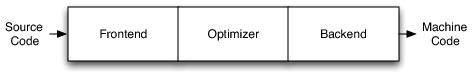
\includegraphics[scale=0.8]{SimpleCompiler.png}
\end{figure}


\section{LLVM}
Az \emph{LLVM} projekt maga is moduláris felépítéssel rendelkezik, sokféle architektúrát és programozási nyelvet képes összekötni. Alkotója Chris Lattner \cite{lattnerhomepage} 2000-ben kezdte meg fejlesztését, azzal a céllal, hogy létrehozzon egy olyan eszköztárat, amely általános, programnyelvtől független értelmezési, fordítási és optimalizációs feladatokat lát el. C++ nyelven íródott, eredetileg C és C++ nyelveket támogatott, 2017-re már több mint 20 nyelvhez léteznek benne megfelelő modulok.
Néhány programozási nyelv, melyre az \emph{LLVM} rendelkezik támogatással:
\begin{AutoMultiColItemize}  
\item C\#
\item Common Lisp
\item Delphi
\item Fortran
\item OpenGL
\item Haskell
\item Java
\item Julia
\item Python
\item R
\item Ruby
\item Rust
\item Scala
\item Swift
\end{AutoMultiColItemize}

\subsection*{IR}
Az \emph{LLVM} projekt, hogy a különböző programozási nyelveket le tudja fordítani a különböző architektúrákra, bevezetett egy köztes reprezentációt. A köztes reprezentáció maga is egy programozási nyelv, hasonlít az assembly-re, erősen típusos. Ennek köszönhetően ha egy új programozási nyelvet szeretnénk lefordítani az eddigi architektúrákra, elég csak egy úgynevezett frontend-et létrehozni hozzá, mely arról gondoskodik, hogy az új programozási nyelvet a köztes reprezentációra alakítja át. Hasonló a helyzet, ha egy új hardvertípust kell támogatni, itt a köztes reprezentációból a gépi kódra átalakító rész neve a backend. A köztes reprezentáció nagy előnye, hogy feloldja azt a skálázási problémát, amit egy új végpont (legyen az egy új nyelv, vagy új architektúra) bevezetése okoz.

\begin{minipage}{\linewidth}
\begin{lstlisting}[caption={Hello World LLVM IR},label=lstlisting:helloworldllvmir]
@.str = private unnamed_addr constant [13 x i8] c"hello world\0A\00"
declare i32 @puts(i8* nocapture) nounwind
define i32 @main() {   ; i32()*
  %cast210 = getelementptr [13 x i8], [13 x i8]* @.str, i64 0, i64 0
  call i32 @puts(i8* %cast210)
  ret i32 0
}

!0 = !{i32 42, null, !"string"}
!foo = !{!0}
\end{lstlisting}
\end{minipage}

\subsection*{SSA}
Az \emph{LLVM} projekt optimalizálási technikák széles körét beveti, hogy hatékonyan tudja a lehető legoptimálisabb kódot generálni. Ezen optimalizációs technikák közül sok épít a köztes reprezentáció egy speciális tulajdonságára, a Static Single Assignment alakra. Az \emph{LLVM}-ben van eljárás az SSA alakra hozásra, és ezt érdemes is megtenni, mert a következő optimalizációs lépések hatékonyabbak:

\begin{AutoMultiColItemize}
\item constant propagation
\item dead code elimination
\item global value numbering
\item register allocation
\end{AutoMultiColItemize}

\section{Clang}
A \emph{Clang} egy frontend, amely a C nyelvi család fordítását végzi. Ennek eredménye az LLVM IR forma. A \emph{Clang} fejlesztése közben emellett az is szempont volt, hogy megfelelő betekintést adjon a fordítás folyamatába, és jó minőségű diagnosztikai információval szolgáljon. Így a \emph{Clang} fordító nem csak a végzetes hibákat jelző üzenetekkel kommunikál a fejlesztő felé, hanem figyelmeztető üzenetekkel is. Emellett a \emph{Clang} forráselemző és forrástranszformációs feladatot is ellát. Ezek a tevékenységek a fordítás során végzett szintaktikus elemzés eredményeit használják fel, így kézenfekvő, hogy a \emph{Clang} keretében kerültek megvalósításra.

\subsection*{Fordító}
A \emph{Clang} elsődleges célja, hogy a C nyelvi család általános fordítójaként használhassák. Ezt a feladatot a kiadásakor legszélesebb körben a GNU Compiler Collection látta el, és még ma is meghatározó a szerepe. A \emph{Clang}-et a fejlesztők úgy alkották meg, hogy a lehető leginkább egy a GCC fordítóval kompatibilis, annak alternatív fordítójaként használható eszköz legyen. Emellett, hogy sok platformon el tudjon terjedni, szüksége van arra, hogy a megfelelő nyelvi forrásfájlokat, illetve programkönyvtárakat fel tudja használni. A legtöbb UNIX alapú rendszer mellett a \emph{Clang} már Windows rendszeren képes akár a natív Visual Studio által kialakított környezettel együttműködni \cite{clangusermanual}.

A GCC-vel való kompatibilitás és az funkciója, hogy képes más fordítási és rendszerkörnyezetekkel együttműködni jelentős többletkomplexitást ad az ,,egyszerű" fordítási feladatához. Emiatt a megvalósítása során több rétegű alkalmazásmodellt választottak a fejlesztők. A \emph{Clang} eszköz a végfelhasználó számára elsődlegesen egy, a platformnak megfelelően lefordított és csomagolt bináris állományként áll rendelkezésre. Ez az eszköz alapértelmezetten a \emph{Clang} driver részét használja, amely meghajtja a fordítási folyamatot. Ez felelős a parancssori opciók feldolgozásáért, a programkönyvtárak és a rendszerhez tartozó forrásfájlok megtalálásáért. Ez a rész az, ami a beérkező parancs és argumentumok együtteséből egy konkrét művelet tervét elkészíti. Lásd \ref{fig:clangdriver}.

A fordítás folyamata 5 fő lépésre tagolható:
\begin{itemize}
\item Parse
\item Pipeline
\item Bind
\item Translate
\item Execute
\end{itemize}

\subsubsection{Parse}
Ebben a fázisban a parancssori argumentumok feldolgozása történik. Az argumentumok tárolása közben megjelenik az a hozzáállás, amely az \emph{LLVM} projektre jellemző, a hatékonyságra törekvés, miszerint minden opció csak egyszer legyen beolvasva, és ne legyen több példányban eltárolva. Ezt a \emph{Clang} driver kódja az opcióknak megfelelő Arg osztály példányainak egy hatékony, központosított tárolóban történő elhelyezésével segíti elő. Ez az ArgList. Ez kihasználja a C nyelvre jellemző string-ábrázolás sajátosságait és  összhangban van C++ nyelv költség nélküli absztrakcióival.

\begin{figure}[h]
\caption{A Clang Driver szerkezete. Forrás \cite{clangdriverimage}}
\centering
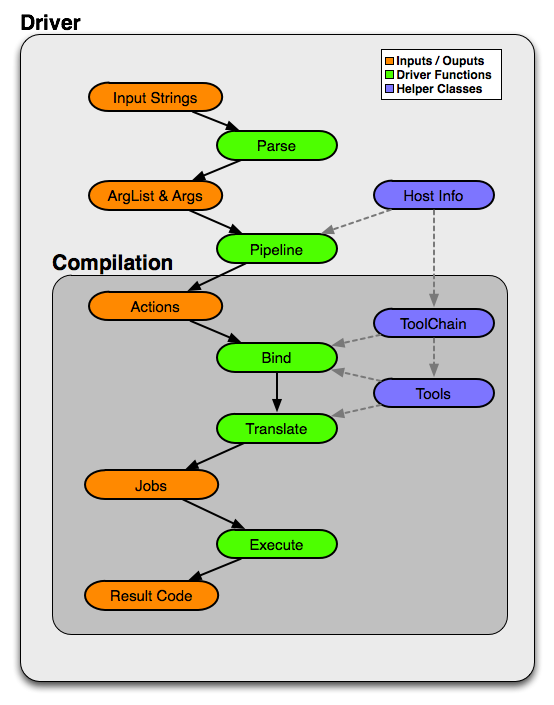
\includegraphics[scale=0.6]{DriverArchitecture.png}
\label{fig:clangdriver}
\end{figure}

\subsubsection{Pipeline}
Miután az argumentumok feldolgozása megtörtént, a fordító megvizsgálja, hogy milyen input és output fájlokkal fog dolgozni a működése során, majd az ezeket összekötő lépéseket nagyvonalakban definiálja. Ezek a lépéseket az Action osztály szimbolizálja a \emph{Clang} driver-en belül. Action példányok egy sorozata ad egy feladatot, Task-ot. A programfordítás során előkerülő eszközök beszédes neveivel jelöli a \emph{Clang} eszköz ezeket az Action lépéseket, például preprocessor, compiler, assembler. Létezik két speciális Action is: az InputAction és a BindArchAction. A fordításhoz kialakított Action lépések listáját a felhasználó meg is tekintheti.

\begin{minipage}{\linewidth}
\begin{lstlisting}[caption={A fordítási pipeline lekérdezése}
\label{lst:driverpipeline}]
clang -ccc-print-phases simple_read.c 
0: input, "simple_read.c", c
1: preprocessor, {0}, cpp-output
2: compiler, {1}, ir
3: backend, {2}, assembler
4: assembler, {3}, object
5: linker, {4}, image
\end{lstlisting}
\end{minipage}

\subsubsection{Bind}
Ebben a lépésben a fordító a kialakított Action sorozatokra próbál meg konkrét megvalósításokat találni. Ezt a ToolChain osztály segíti, amely eszközöket, Tool-okat tartalmaz. A Tool-ok végzik el a konkrét fordítási fázis egy-egy folyamatát. A fordító először megkeresi melyik ToolChain melyik Tool-ja szükséges egy Action végrehajtásához, majd a későbbiekben a fordító a Tool-lal kommunikálva újabb folyamatokat szúrhat be a végrehajtási listába.

\begin{minipage}{\linewidth}
\begin{lstlisting}[caption={A fordítási tool-ok lekérdezése}
\label{lst:driverbind}]
clang -ccc-print-bindings -arch i368 simple_read.c
# "x86_64-unknown-linux-gnu" - "clang", inputs: ["simple_read.c"], output: "/tmp/simple_read-3c1f07.o"
# "x86_64-unknown-linux-gnu" - "GNU::Linker", inputs: ["/tmp/simple_read-3c1f07.o"], output: "a.out"
\end{lstlisting}
\end{minipage}

\subsubsection{Translate}
Miután a fordító kiválasztott egy eszközt, az eszköz feladata, hogy Command típusú objektumokat állítson elő. Ezek a ténylegesen futtatandó alfolyamatokat, és argumentumaikat szimbolizálják. A legtöbb munka azzal van, hogy a GCC-vel kompatibilis opciókat a Tool lefordítsa a futtatandó eszköz számára értelmezhető beállításokká. Sok helyen ez nem bonyolult, az assembler például tipikusan kevés külső opcióval dolgozó program, de a linkerek ezzel szemben argumentumok széles skáláját használják aktívan \cite{clangdriverinternals}.

\subsubsection{Execute}
A fordítás végrehajtása a driver számára a legegyszerűbb lépés, kevés opcióval, van azonban lehetőség a programkimenetek átirányítására, az egyes eszközök visszatérési értékeinek továbbadására, illetve a folyamatok teljesítménymérésére is.

\subsection*{Elemző}
A \emph{Clang} eszköz alapértelmezetten megpróbál segítséget nyújtani a fordítás során akkor is, ha külön nem kérjük rá. A fordításkor felmerülő hibaüzenetek mellett figyelmeztetőüzenet széles skáláját használja ahhoz, hogy az esetleges hibák, nem várt működések kiküszöbölésében segítse a programozót.

A fordítás közben kiadott hibaüzenetek és figyelmeztetések mellett lehetőség van más vizsgálatok lefuttatására is, amelyek a tüzetesebb vizsgálatnak vetik alá a programot. Ezek általában valamilyen futás, vagy fordításidejű költséggel rendelkeznek, ezért a közönséges fordítás alatt nem futnak le alapértelmezetten.
A \emph{Clang} és \emph{LLVM} infrastruktúra több ilyen módszerrel is bír. A különböző Sanitizer névre hallgató megvalósítások, például AddressSanitizer, MemorySanitizer, UndefinedBehaviorSanitizer lényege, hogy a program lefordításakor a keletkező bináris állományban a program futása mellett a program működését vizsgáló logika is fut, és hiba érzékelése esetén fájlban vagy sztenderd kimeneten értesítést erről. Ezek futásidejű hibakeresési módszerek. Dolgozatomban a forráselemzés által felfedhető hibák detektálásával foglalkozom, így a \emph{Clang} eszköznek ezen részeit ismertetem a továbbiakban.

Hogy a \emph{Clang} fordító és a \emph{Clang} driver kapcsolatát jobban megérthessük nézzük meg az absztrakt szintaxisfa (AST, abstract syntax tree) kinyomtatásához felhasznált parancsot (lásd kódrészlet \ref{lst:astdump}). A következő két parancs ugyanazt az Action-t adja, és ugyanazt az analízismodulhoz tartozó műveletet indítja el. Az egyetlen különbség, hogy a második nem megy végig a driver előfeldolgozó részén, és így az esetleges rendszerhez tartozó header fájlok nem láthatóak a fordítónak, azokat a GCC esetében már megismert -I és -isystem kapcsolókkal megadhatjuk (valójában ezt teszi a driver is).

\begin{lstlisting}[caption={A driver és a compiler közvetlen kapcsolata}
\label{lst:driverandcompiler}]
//driver
clang --analyze -Xanalyzer -ast-dump file_read.c
//clang-frontenden
clang -cc1 -analyze -ast-dump file_read.c
\end{lstlisting}

\subsubsection{Integrációs lehetőségek}
A \emph{Clang} könyvtárcsomag számos diagnosztikai információt tud szolgáltatni a C nyelvcsalád programjaival kapcsolatban. Amikor forráskódelemzést végzünk, akkor a \emph{Clang} fordítónak általában csak az előfeldolgozó (a driver), és a szintaxisfa felépítéséért felelős részét használjuk. A köztes reprezentációra alakítás, illetve az ebből történő tárgykód-előállítás elmarad. Ennek fő oka, hogy a hibák detektálásához a legtöbb statikus analízist bevető megoldás a vizsgált nyelv sajátosságait használja fel, míg az általános IR reprezentációban szereplő esetleges nem várt, vagy nem hatékony működéseket az optimalizációs lépés küszöböli ki. Így nincs tehát szükségünk statikus analízis vizsgálatok lefuttatásához az IR-re, megállhatunk a kész szintaxisfa szintjén.

Ezt a szintet engedi vizsgálni a \emph{Clang} könyvtár három fő interfészén keresztül, amelyet a \emph{Clang}et felhasználó fejlesztők rendelkezésére bocsát. A főbb felületek:
\begin{itemize}
\item LibClang
\item LibTooling
\item Clang Plugin
\end{itemize}

\subsubsection{LibClang}
A \emph{Clang} fejlesztői fontosabbnak tartják a hatékonyságot szem előtt tartó folyamatos átalakításokat, illetve az új funkciók minél hamarabbi bevezetését, mint a szigorúan betartott visszafele-kompatibilitást, amikor a kódbázisról van szó. Ennek köszönhetően hatékony szoftvert kapunk, amikor a \emph{Clang}-et használjuk, de ez a fejlesztőktől aktívabb közreműködést vár el, amikor egy \emph{Clang} belső reprezentációval rendelkező szoftvert kell fenntartaniuk. Ez főleg a szintaxisfát érinti, amikor egy új \emph{Clang} verzióban a szintaxisfa reprezentációja megváltozik, vagy esetleg új nyelvi elemeket emelne be, akkor egy régebbi \emph{Clang} verzióval kompatibilis könyvtár elromolhat az új verzióban. Akik egy stabilabb fejlesztési felületre vágynak, azoknak megfelelő a LibClang interfész. A LibClang egy C nyelven írt könyvtár, amely bár nem biztosítja az AST-hez való közvetlen  hozzáférést, ezt áldozza fel a stabilitás kedvéért.

A LibClang könyvtár emellett a megszorítás mellett is sok területen kedvelt és használt. Ennek a segítségével megvalósítható a \emph{Clang} által kezelt nyelvek forráskód szintű vizsgálata. Lehetőséget a szintaxisfa bejárására a látogató (visitor) programozási minta segítségével, így relatíve magas absztrakciós szinten ad lehetőséget a forráskód statisztikai elemzésére (pl. használt nyelvi elemek száma, előfordulási sűrűsége egyes modulokon belül, más elemekkel együtt való használat gyakorisága stb.), intelligens kontextusvizsgálatra, illetve nyelvi konstrukciók forráskódbeli helyükkel való pontos összekötésére \cite{libclangdocs}. Ezen funkciók kihasználása teszi lehetővé, hogy olyan eszközöket készítsünk a LibClang felhasználásával, mint automatikus forráskódformázó eszközök, amelyek egy kódstílust leíró konfiguráció segítségével tetszőleges forrásállományt át tudnak formázni úgy, hogy csak külalakra változik, struktúrája azonban ugyanaz marad. Emellett képesek lehetünk automatikus kódkiegészítők alkotására, melyek integrált fejlesztői környezetekben (IDE) kontextusfüggően képesek javaslatokat tenni a szerkesztés alatt levő forráskódokra. Emellett a LibClang könyvtár nagy előnye a másik két lehetőséggel szemben, hogy mivel C nyelvi interfész, ezt lehet a legkönnyebben más, akár dinamikusan típusos script-nyelvek programjaiba is integrálni. Python nyelvre van a hivatalosan nyilvántartott dokumentációban is hivatkozás, mint ahogy arra is, hogy az XCode IDE az OSX rendszeren használja ezt a lehetőséget \cite{clangtooling}.

\subsubsection{LibTooling}
A LibTooling interfész C++ nyelvet használ, emiatt sokkal természetesebb módon, nagyobb manipulációs lehetőséget biztosít az AST-t tekintve, mint a LibClang. Elsődlegesen különálló alkalmazások fejlesztésére tervezték. Megvan a LibClang könyvtár ismertetésekor felhozott hátránya, miszerint a \emph{Clang} szintaxisfa-reprezentációinak változásakor könnyen visszafele-kompatibilitási problémák léphetnek fel. Emellett a közvetlen szintaxisfa közvetlen elérése lehetőséget ad arra, hogy bonyolultabb átalakításokat végezzünk forráskódokon. Nem csak kozmetikai változások lehetségesek, hanem akár ekvivalens, vagy valamilyen tulajdonságot megtartó strukturális átalakítások is (pl. refaktorálás vagy obfuszkálás). Emellett természetesen rendelkezésünkre áll minden, ami LibClang használata esetében is, így nagyon pontos a nyelvi elemek és forráskódbeli pozíciójuk közötti leképezés, tehát forrás-diagnosztika szoftverek alapjául is szolgálhat.

\subsubsection{Clang Plugin}
A \emph{Clang} modulárisan felépített szoftver, lehetőséget ad a kiterjesztésre. A Clang Plugin rendszer segítségével a fordítás közben különböző műveleteket végezhetünk a szintaxisfán. Ezek a művelet többek között analitikai műveletek is lehetnek, a Clang Static Analyzer (Clang SA) projekt is ezt a megoldást választotta a különböző problémákat felismerő ellenőrző modulok (checker-ek) futtásához. Lehetőség van statikus linkelésű checkerek, illetve dinamikus linkelésű beépülő modulok létrehozására is. A Clang SA alapvetően statikusan linkelt checker-eket használ. A Plugin rendszer hátránya a LibTooling-hoz képest, hogy alapvetően a fordítási folyamat részeként fut az ellenőrzés, emiatt a build-rendszer vezérli, és így egyetlen különálló forrásfájl magában nem igazán támogatott. Sokkal idiomatikusabb, és egyszerűbb ennél az eszköznél egy egész projekt elemzése. Tipikusan Plugin-t használnak még a fordítási figyelmeztetéseket adó, illetve a build-folyamat során járulékos állományokat létrehozó modulok.

\subsubsection{Clang Static Analyzer}
A Clang Static Analyzer egy forráselemző, amellyel C, C++, Objective-C programok hibáit lehet megtalálni. Alapvetően parancssori eszköz, azonban hivatalos integrációja létezik az Apple XCode fejlesztői környezettel, ahol alapértelmezetten be van építve. Használata inkább kötődik a kód fordítását végző build-folyamathoz, ekkor nem egy-egy forrásfájlról ad hibainformációkat, hanem egy egész projektről, de emellett lehetőség van egyszeri fordítás ellenőrzött elvégzésére is.

\begin{figure}[h]
\caption{Clang Static Analyzer hibainformációk. Forrás \cite{clangsaimage}}
\centering
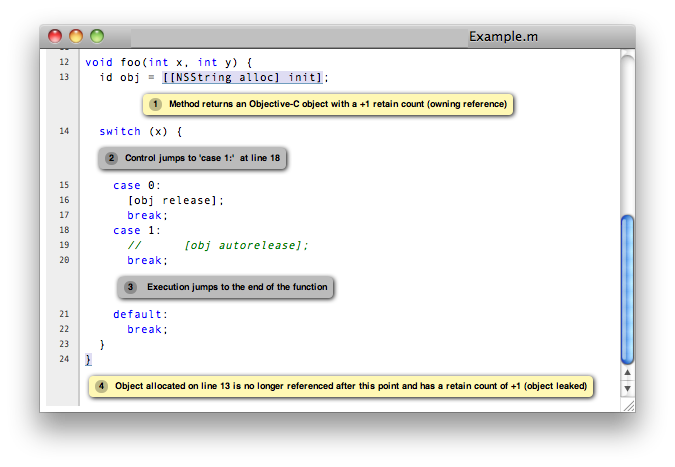
\includegraphics[scale=0.6]{analyzer_html.png}
\end{figure}

Alapvetően a használatához szükség van a \emph{Clang} forráskódjával csomagolt scan-build és scan-view eszközökre, de elérhető bináris formában OSX rendszerre is \cite{clangsahomepage}. A scan-build alapvetően perl nyelven íródott, de egy modernebb megvalósítása elérhető Python nyelven is, ennek használatát javasolják a fejlesztők új projektek esetében.

\begin{figure}[h]
\caption{A scan-build-py eszköz parancssori futása.}
\centering
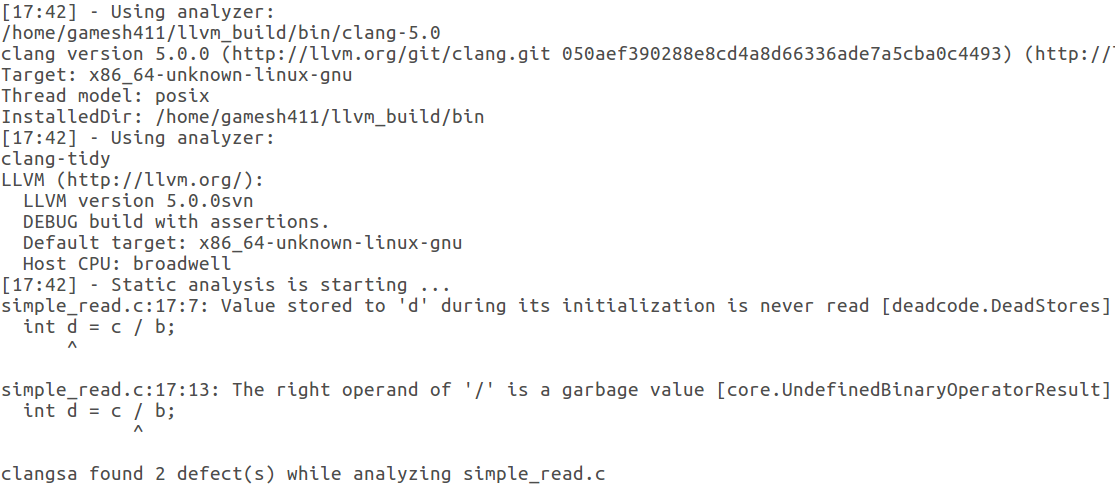
\includegraphics[scale=0.4]{uninit_commandline.png}
\end{figure}

A parancssori futás eredményét egy webes felületen megtekinthetjük, a scan-build-py eszköz html fájlok formájában is eltárolja egy-egy futás eredményét. A scan-view alkalmazás megtalálja az elemzés eredményét és megmutatja.

\begin{figure}[h]
\caption{A scan-build-py eszköz eredményeinek webes megjelenítése.}
\centering
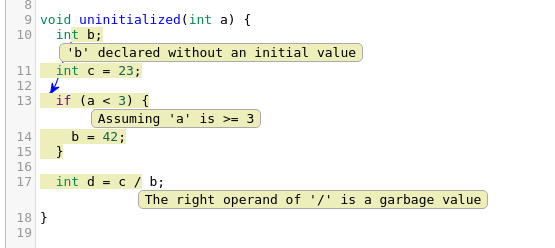
\includegraphics[scale=0.8]{uninit_web.png}
\end{figure}

Az eszköz már magában is képes teljes értékű elemző, azonban a megvalósított program az Ericsson által fejlesztett \emph{CodeChecker} \cite{codecheckergit} alkalmazást használja, amely kifinomultabb, jobb kezelhetőséget, és felhasználói élményt biztosít az ellenőrzések futtatására.

\chapter{Checkerek}
A Clang SA egy keretrendszer, amely a képes a checker-ek futtatására. Két féléves gyakorlatom során, amit az Ericsson csapatával töltöttem két checker-t implementáltam. Az egyik a C++ nyelvi I/O könyvtár, a stream-ek helyes használatával foglakozik, a másik egész számtípusokon végzett típuskonverziókkal.
Ha egy checker már a \emph{Clang} része, akkor közvetlenül is futtathatjuk a parancssorból, használhatjuk a Clang SA scan-build, vagy scan-build-py eszközöket, vagy ezekre épülő eszközöket, például az Ericsson által fejlesztett \emph{CodeChecker}-t.

\begin{lstlisting}[caption={Clang SA Checker futtatása közvetlenül}
\label{lst:checkerdirectrun}]
clang -cc1 -analyze -analyzer-checker=<name of checker to run> <source files>
\end{lstlisting}

\section{Fejlesztői útmutató Checker-ekhez}
A Checker-ek az \emph{LLVM}, ezen belül a \emph{Clang} eszköz forráskönyvtárában helyet foglaló C++ állományok és néhány bejegyzés, amelyek felfedezhetővé teszik a build-rendszer számára az új Checkert. Hogy egy Checkert hozzá tudjunk adni a \emph{Clang} fordítóhoz, meg kell szereznünk az \emph{LLVM} és \emph{Clang} forrást \cite{getllvmpage}.

\begin{lstlisting}[caption={Clang beszerzése GitHubról.}
\label{lst:getllvm}]
git clone http://llvm.org/git/llvm.git
git clone http://llvm.org/git/clang.git llvm/tools/clang
\end{lstlisting}

Az \emph{LLVM} projekt cmake build-rendszerrel rendelkezik, és ezen túl egy tablegen eszköz még részt vesz a build folyamatban. Tegyük fel, hogy egy új Checker-t szeretnénk hozzáadni. Legyen a neve ExampleChecker.

Ekkor létre kell hoznunk egy implementációs fájlt a forrásfán belül az llvm/tools/clang/lib/StaticAnalyzer/Checkers könyvtáron belül ExampleChecker.cpp névvel.

Láthatóvá is kell tennünk a cmake build-rendszer számára az által, hogy bejegyezzük a többi Checker forrásfájljainak neve közé a llmv/tools/clang/lib/StaticAnalyzer/Checkers/CMakeLists.txt-ben.

Az implementáció mellett szerepelnie kell egy regisztrációs kódnak.

\begin{lstlisting}[caption={Checker beregisztrálása. Forrás \cite{checkerdevmanual}}
\label{lst:checkerregistration}]
void ento::registerExampleChecker(CheckerManager &mgr) {
  mgr.registerChecker<ExampleChecker>();
}
\end{lstlisting}

Az előbbi \ref{lst:checkerregistration} regisztrációs kód megköveteli, hogy az implementáció logikáját tartalmazó osztály neve ExampleChecker legyen.

Az llvm/tools/clang/lib/StaticAnalyzer/Checkers/Checkers.td fileban kell még bejegyeznünk a checker-ünket ahhoz, hogy a tablegen megtalálja.

\begin{lstlisting}[caption={Checker beregisztrálása tablegen eszköz számára. Forrás \cite{checkerdevmanual}}
\label{lst:checkerregistrationtablegen}]
let ParentPackage = "{{where the checker belongs}}" in {
...
def ExampleChecker : Checker<"Example">,
  HelpText<"{{ExampleChecker help text}}">,
  DescFile<"ExampleChecker.cpp">;
...
} // end "{{where the checker belongs}}"
\end{lstlisting}

Miután a Checker-t implementáltuk, megkezdhetjük a \emph{Clang} fordítását. A fordítást érdemes egy külön könyvtárban végezni, így lehetőségünk van ugyanannak forrásfának más és más konfigurációit is megépíteni és kipróbálni.

\begin{lstlisting}[caption={A Clang fordítása}
\label{lst:buildingclang}]
mkdir clang_build
cd clang_buidl
cmake ../llvm
make
\end{lstlisting}

Az \emph{LLVM} és a \emph{Clang} nagy projektek, sokáig tarthat a fordítás, és a linkelés fázisában sok memóriára van szükség. Ezeken a problémákon segíthetünk ha például a legtöbb Linux rendszerben elérhető gold linkert használjuk, amely kisebb memóriaigénnyel bír, így akár több folyamatot is indíthatunk, amikor a \texttt{make} parancsot kiadjuk (például \texttt{make -j4}).

A fordítási folyamat felgyorsítása érdekében használhatjuk a ninja nevű build-rendszert, ehhez telepítenünk kell a ninja csomagot, és az általunk kiadott a cmake parancsban a \texttt{-GNinja} kapcsolót is meg kell adnunk.

Az is csökkenti a fordítási időt, hogy ha nem minden architektúrára építjük meg a kódgeneráláshoz szükséges könyvtárakat, csak a futtató környezet natív célpontjára. Ez az elterjedt X86-os architektúra esetében például a \texttt{-DLLVM\_TARGETS\_TO\_BUILD="X86"} kapcsolóval lehetséges.

Ha sikeres a fordítás, akkor a keletkező \emph{Clang} futtatható állomány segítségével ellenőrizhetjük, hogy minden rendben van-e, vagyis, hogy látjuk-e a checker-ek között a sajátunkat. Más projektekhez hasonlóan a keletkezett futtatható állományokat használhatjuk közvetlenül a build-könyvtárból, vagy az \texttt{install} cél megépítésével behelyezhetjük őket a rendszerkönyvtárak közé.

\begin{lstlisting}[caption={A Clang checkerek kilistázása}
\label{lst:listclangcheckers}]
clang -cc1 -analyzer-checker-help
\end{lstlisting}

\section{OStreamFormatChecker}
Az OStreamFormatChecker a C++ nyelvi könyvtárat ellenőrzi, és segítségével meg lehet találni olyan kódrészleteket, amelyek átállították egy \texttt{std::ostream} típusú, írható, vagyis kimeneti stream formázási állapotát, de utána nagy valószínűséggel elfelejtették ezt visszaállítani.

\subsection{Specifikáció}
A problémát egy mintakóddal specifikáljuk, mely során a kódsorokban kommentek formájában jelezzük, hogy az elvárt működés szerint ott hibát kell-e adnia checker-nek vagy nem. Ehhez hasonló rendszert használ az \emph{LLVM} projekt beépített tesztelő keretrendszere is, tehát a checker-hez tartozó tesztelő kódomban is ilyen formátumban jeleztem, ha valahol elvárt jelenség az, hogy hibát jelezzen a checker.

\begin{lstlisting}[caption={OStreamChecker specifikációja}
\label{lst:ostreamcheckerspec}]
class StreamState {
public:
  StreamState(std::ostream& out)
  : m_out(out), m_fmt(out.flags()), m_prec(out.precision()) {}

  ~StreamState() {
    m_out.precision(m_prec);
    m_out.flags(m_fmt);
  }

private:
  std::ostream& m_out;
  std::ios_base::fmtflags m_fmt;
  std::streamsize m_prec;
};


void test1(int i) {
  std::cout << std::hex << i;  //err stream format state is not restored to dec
}

void test2(int i) {
  std::cout << std::hex << i <<dec;  //ok
}

void test3 (int i) {
  std::cout << setprecision(2) << i; //err stream state changed, but not restored
}

int test4 () {
  std::cout.setf ( std::ios::hex, std::ios::basefield );  // set hex as the basefield
  std::cout.setf ( std::ios::showbase );                  // activate showbase
  std::cout << 100 << '\n';
  std::cout.unsetf ( std::ios::showbase );                // deactivate showbase
  std::cout << 100 << '\n';
  return 0; //err format flag set to hexadecimal, but not restored
}

void test5(int mv) {
  StreamState ss(cout);
  std::cout << std::setiosflags(std::ios::fixed) << std::setprecision(6); //std::cout stream state is set here
  std::cout << "Maurer Randomness Test returned value " << mv << endl;
}//OK std::cout stream state is recovered here
\end{lstlisting}

Látható, hogy ez a checker a globális státuszinformációt tartalmazó, \texttt{std} névtérben lévő, sztenderd kimenetet szimbolizáló stream objektum elfelejtett módosításait detektálja. Abban az esetben, ha egy függvényben történt módosítás az \texttt{std::cout} formázóállapotában, akkor hibát kell jeleznünk, abban az esetben viszont, hogy ha a formázás értékét visszaállítjuk mielőtt véget ér a függvény futása, akkor helyesen használták a stream-et.

Külön érdekesség, hogy ha a C++ nyelvi rendszerét kihasználó destruktor hívásban történik a visszaállítás, akkor sem akarunk hibát kapni, hiszen az élettartamszabályok értelmében a \texttt{test5} függvény esetében az \texttt{ss} lokális változó élettartama véget ér függvény végén, és meghívásra kerül a destruktora, amely visszaállítja a formázók állapotát.


\section{EnumCastOutOfRangeChecker}
Az EnumCastOutOfRangeChecker egy, a SEI CERT C++ Coding Standard által megfogalmazott problémára jelent egy megvalósítást \cite{securecodingint50}.
A C illetve C++ nyelv is rendelkezik enumeráció (felsorolási) adattípussal, amely képes arra, hogy emberek által jól megjegyezhető szöveges formában kódolható fogalmakat feleltessen meg egész típusú értékeknek. Így ha egy kategória jól körülhatárolható elemekkel és véges elemszámmal rendelkezik, akkor ésszerű lehet ezt a kategóriát a programozási nyelv szintjén egy enumerációval ábrázolni. Kiválóan alkalmasak interprocedurális, illetve hálózati kommunikációra is, hiszen az őket definiáló forráskódnak kell rendelkezésre állni mindkét oldalon az egyértelmű kódolás és dekódolás megvalósításához.

\begin{lstlisting}[caption={Enumerációs típusok tipikus felhasználása.}
\label{lst:enumdemo}]
enum Nap { Hetfo, Kedd, Szerda, Csutortok, Pentek, Szombat, Vasarnap };
\end{lstlisting}

Lehetőség van C-ben és C++-ban is, hogy bármilyen megfelelő egész típusú értéket enumeráció típusúvá alakítsunk, a típuscserét sokszor valamilyen explicit konverzió (cast), segítségével érhetjük el. Abban az esetben viszont, amikor egy olyan egész értéket szeretnénk egy enumeráció típusba kényszeríteni, amelyik nem reprezentál egy valódi enumeráció értéket sem, nem definiált a keletkezett érték.

Mivel ez a probléma a típusrendszerhez köthető, felfedezése eleve nehézségekbe ütközik, ha futásidőben próbálnánk meg, hiszen olyan esetben már egy nem definiált értéket kellene vizsgálnunk. Ezen pedig szinte minden összehasonlító művelet szintén nem definiált eredményt ad. Tehát ennek a problémának a felderítése tipikusan a statikus analízis eszköztárát követeli meg.

Egy enumerációs típus értékei elég különlegesek is lehetnek, használatuk sokszor előfordul template metaprogramozás esetén.

\begin{lstlisting}[caption={Különleges enum értékek.}
\label{lst:specialenumvalues}]
template <int N>
struct Factorial
{
  static const int val = N * Factorial<N - 1>::val;
};

template <>
struct Factorial<0>
{
  static const int val = 1;
};

enum dummy { a = 4, b = 8, c, d = 3, e = Factorial<5>::val };
\end{lstlisting}

Ebben a példában a C++ nyelvi sajátosságait felhasználva fordításidőben kerül kiszámításra a faktoriális értéke. Külön érdekesség, hogy itt a rekurzió alapesetének definiálása egy template-specializációval történik.


\subsection{Specifikáció}
A probléma specifikálása több részletben történik \cite{securecodingint50}, először egy potenciálisan hibás esetet mutat be, amelyben megtörténik a típuskonverzió, és potenciálisan nem definiált az eredménye.

\begin{lstlisting}[caption={EnumOutOfRangeChecker potenciálisan hibás specifikációja}
\label{lst:enumcastpotentialerror}]
enum EnumType {
  First,
  Second,
  Third
};
 
void f(int intVar) {
  EnumType enumVar = static_cast<EnumType>(intVar);
 
  if (enumVar < First || enumVar > Third) {
    // Handle error
  }
}
\end{lstlisting}

A következő specifikáció egy mindenképpen helyes használatot vázol fel, erre semmiféleképpen nem szabad hibát jeleznie a checker-nek.

\begin{lstlisting}[caption={EnumOutOfRangeChecker potenciálisan hibás specifikációja}
\label{lst:enumcastok}]
enum EnumType {
  First,
  Second,
  Third
};
 
void f(int intVar) {
  if (intVar < First || intVar > Third) {
    // Handle error
  }
  EnumType enumVar = static_cast<EnumType>(intVar);
}
\end{lstlisting}

Emellett vannak még esetek, ahol nem szükséges hibát adnunk. Ezekben az esetekben viszont vagy C++11-es enumerációkról van szó, vagy fix háttértípussal rendelkezőekről. A checker azonban szimbolikus végrehajtást használva jelenleg abban az esetben ad hibát, ha egyértelműen kiderül, hogy az érték, amire a típuskonverziót alkalmazzuk egyértelműen nincs benne az enumeráció értékkészletében. Azért használ ilyen konzervatív feltételt, hogy el tudja kerülni a hamis pozitív jelzéseket.

\chapter{Felhasználói dokumentáció}
A CheckRunner egy grafikus felülettel rendelkező szoftver, mely képes a \emph{Clang} eszköz által támogatott checker-ek segítségével statikus analízis futtatására, és az eredmények megtekintésére. Mindezt a felhasználó egy jól kezelhető, áttekinthető felületen teheti. Célja, hogy demonstrálja a statikus analízis megvalósításának lehetőségit. A \emph{CodeChecker} eszközzel való laza, de mégis hatékony összekötés bemutatja a statikus analízist támogató eszközök együttműködési képességeit, és hatékony segítsége lehet a C nyelvi család tagjaival foglalkozó szoftverfejlesztőknek.

\section{CodeChecker}
A CodeChecher projekt az Ericsson által fejlesztett nyílt forráskódú, dinamikusan fejlődő és hatékony eszköz, amely nem csak a Clang SA hanem a Clang Tidy elemzővel is együtt tud működni. Robosztus és felhasználóbarát felületet ad az analízis végrehajtására, és az eredmények megtekintésére. Emellett képes az eredmények összehasonlítására, rendezésére is.

\begin{figure}[h]
\caption{CodeChecker architektúra. Forrás \cite{codecheckerslide}}
\centering
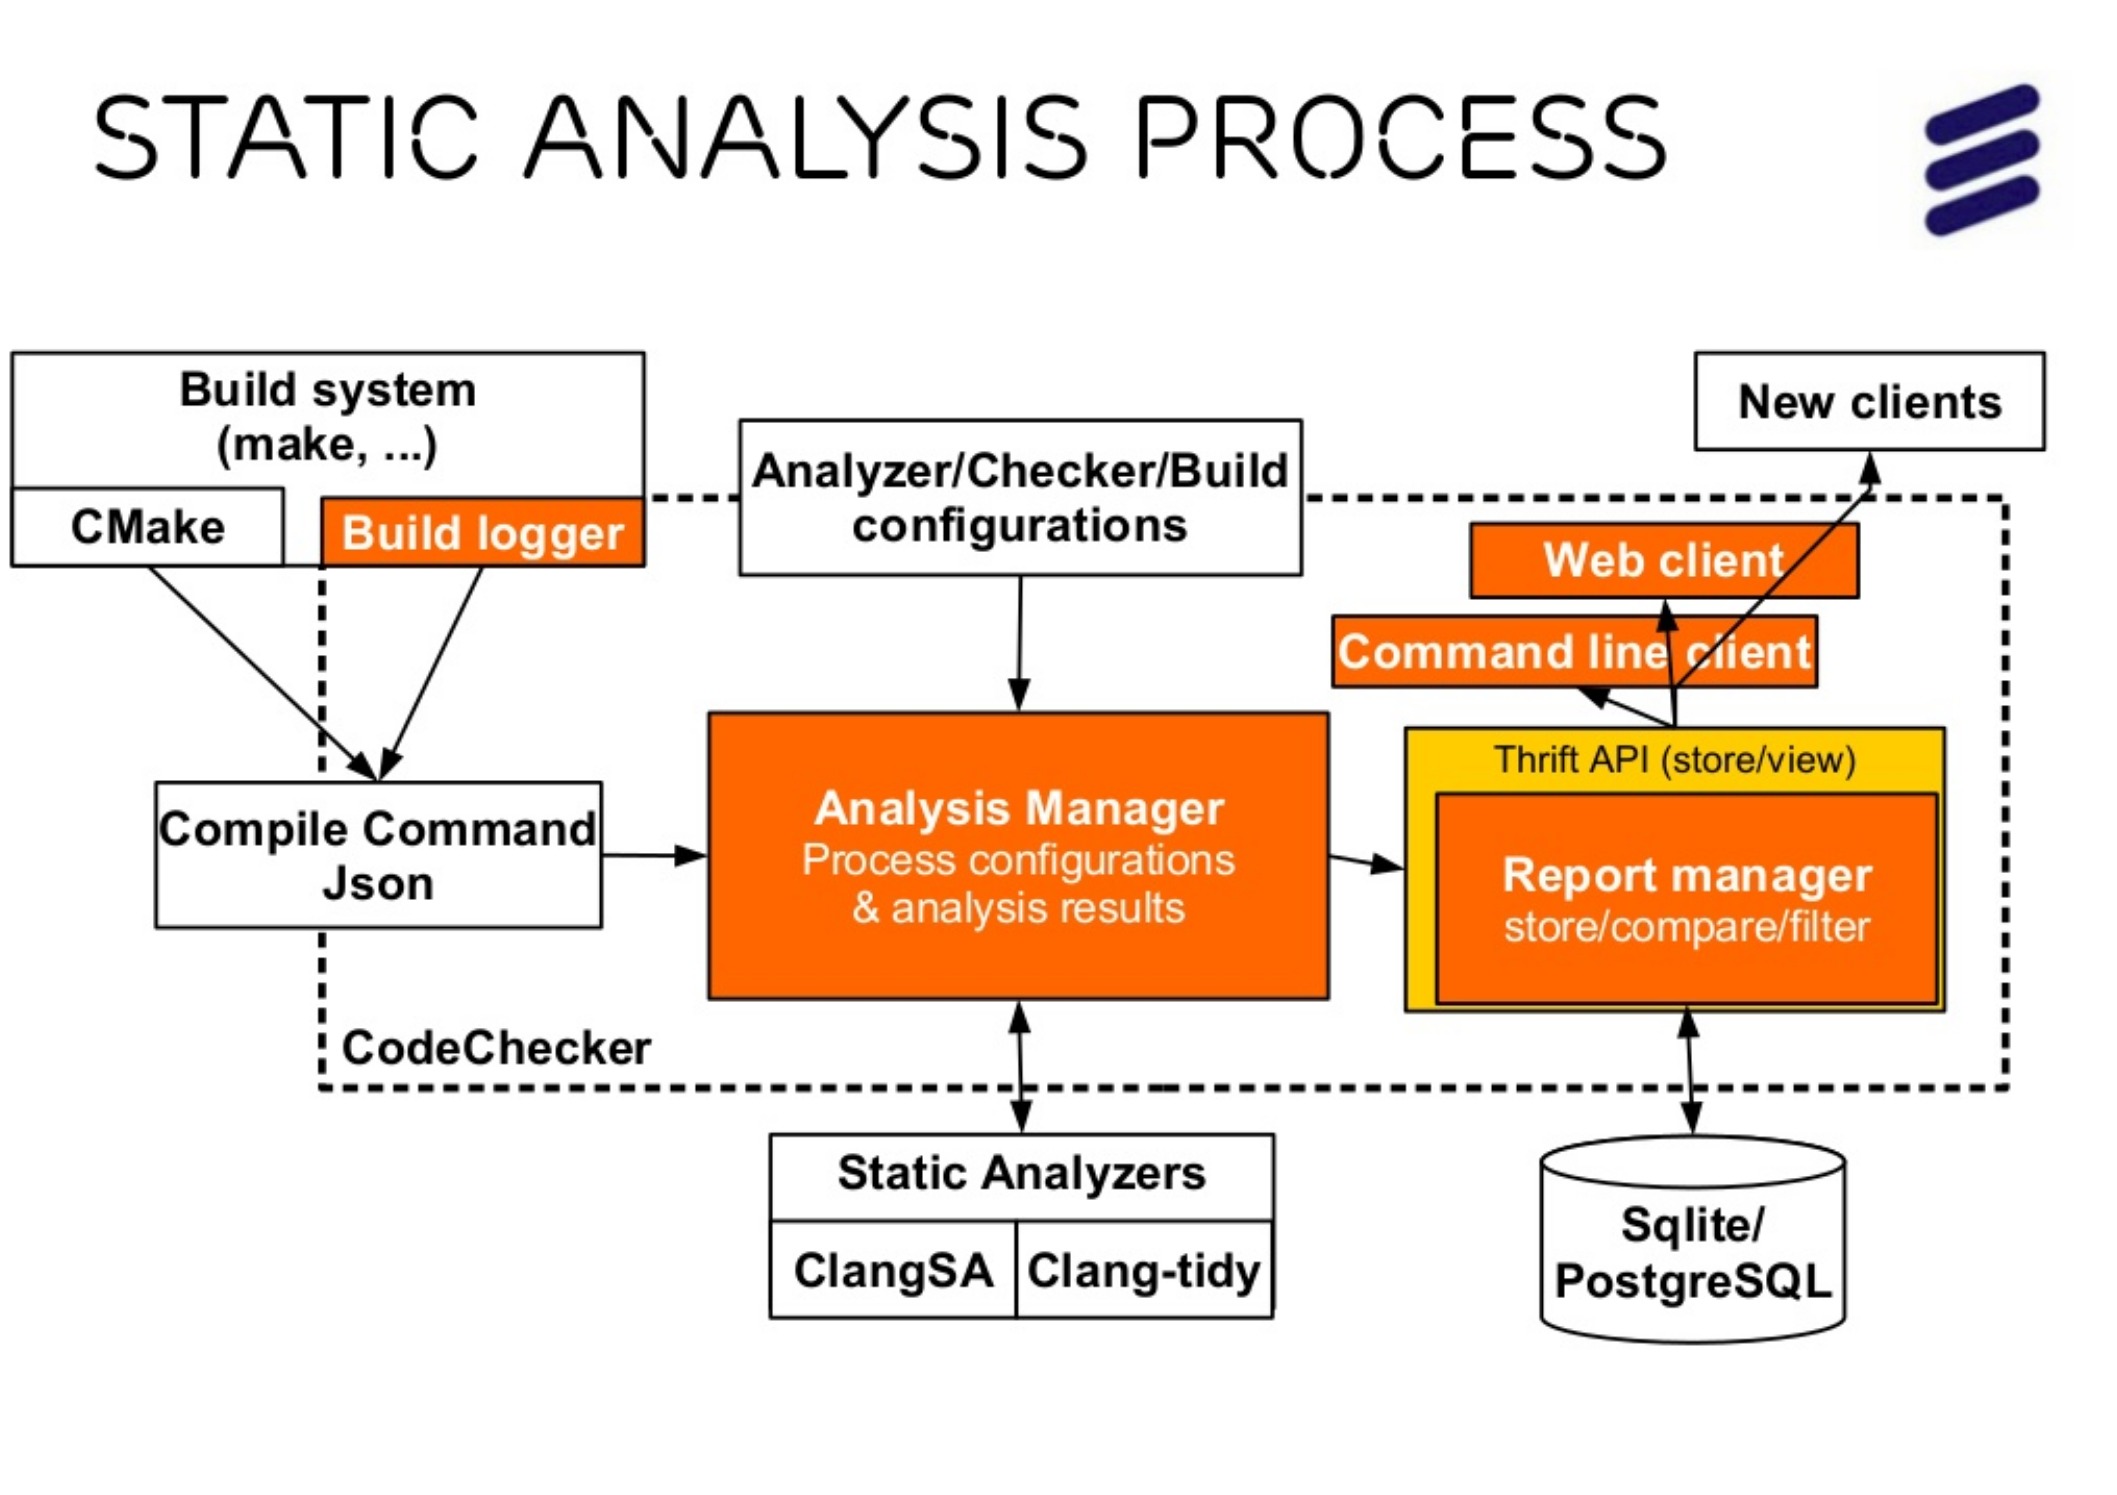
\includegraphics[scale=0.2]{codechecker.png}
\end{figure}

\section{Rendszerkövetelmények}
A felhasznált eszközök technikai hátteréből kifolyóan UNIX alapú rendszereken képes hatékonyan futni a mögöttes keretrendszer, illetve a \emph{CodeChecker} szoftver is. Ebből kifolyólag a program futtatásához egy Linux Ubuntu 16.04 LTS 64 bites operációs rendszer szükséges AMD64 (más néven X86-64) architektúrás processzorral ellátott PC-vel.

\section{Telepítés}
A futtatáshoz szükséges a Python programnyelvi környezet 3-as verziója, emellett a CodeChecker szoftver függőségei. A szakdolgozat írásakor elérhető Ubuntu 16.04-es verziójú Linux disztribúció beépített Python 3.5.2-es verzióján teszteltem a szoftver.

Egy ilyen összeállítás mellett a mellékleten található checkrunner mappát kell tetszőleges helyre átmásolni. A mappa tartalmazza a \emph{CodeChecker} 5.7.1-es verzióját a \texttt{codechecker} mappában. Használat előtt a \emph{CodeChecker} oldalán dokumentált függőségeket a csomagkezelőből telepíteni kell.

\begin{lstlisting}[caption={CodeChecker függőségei.}
\label{lst:codecheckersytemdeps}]
# Install mandatory dependencies for a development and analysis environment
# NOTE: clang-3.8 can be replaced by any later versions of LLVM/Clang
sudo apt-get install clang-3.8 build-essential curl doxygen gcc-multilib \
  git python-virtualenv python-dev thrift-compiler
\end{lstlisting}

Ezután a könyvtárban található \texttt{install.sh} script segítségével lehet telepíteni a CodeCheker-t, és magát az alkalmazást is. Internetkapcsolat szükséges, mert a Python csomagkezelő, illetve a CodeChecker egyedi függőségeinek feloldása is megköveteli. A \emph{CodeChecker} alapértelmezetten a függőségek között feltelepített clang-3.8 -as verziót használja, de természetesen lehetőség van felhasználó által összeállított könyvtár használatára is. Ennek lépéseit már ismertettem a dolgozat első felében a 3.1-es fejezetben. Ha az aktuális felhasználó home könyvtárában végeztük az ott szereplő lépéseket, akkor a program már alapértelmezetten azt használja, elősegítve a fejlesztői környezet gyors összeállítását. Ha esetleg más könyvtárban tároljuk a lefordított \emph{LLVM} és \emph{Clang} komponenseket, akkor a használni kívánt könyvtárat a \texttt{codechecker-wrapper} állományban állíthatjuk be.

\section{Használat}
A programot a \texttt{checkrunner.sh} állomány segítségével indíthatjuk el. A grafikus felület indításakor a program kezelőfelületén láthatjuk az aktuálisan használt \emph{Clang} eszközben regisztrált checker-eket a bal felső részen. A felület lehetőséget biztosít arra, hogy csak bizonyos checker-eket futtassunk le. Ez kifejezetten hasznos, amikor tesztelni szeretnénk egy általunk fejlesztett modult. A modulok neve szerepel a felsorolásban, amelyek mellett pipálható dobozok (checkbox-ok) segítségével érvényesíthetjük a választásunkat.


\begin{figure}[h]
\caption{A felhasználói felület futás közben.}
\centering
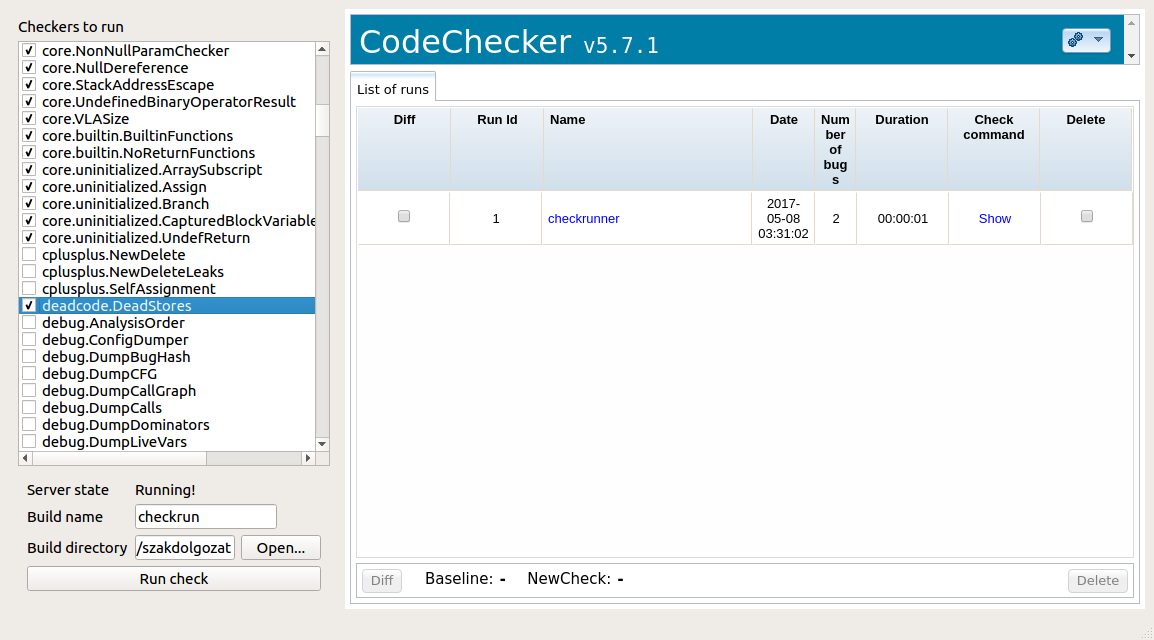
\includegraphics[scale=0.36]{ui.png}
\end{figure}

A felhasználói felület indításakor automatikusan elindítja a CodeChecker beépített adatbázis, és webszerver komponensét, és ezen komponensek folyamatos működése előfeltétele a program működésének. A felület bal alsó részén található egy indikátor, mely a háttérben futó adatbázis, és webszerver állapotát hivatott mutatni. ha \emph{Running!} szöveg szerepel, akkor fut, és ebben az esetben lehetőség van a használat megkezdésére. A következő sorban megadhatjuk az analízis nevét, ezzel tudjuk megtalálni a későbbiekben. A következő sorban meg kell adnunk azt az útvonalat, amely az elemzésre váró projekthez tartozik. Megkötés, hogy csak olyan projektmappát választhatunk ki, amely rendelkezik egy \texttt{Makefile} állománnyal. Ha esetlegesen nem a GNU Make alkalmazás segítségével működik a build rendszerünk, akkor sok esetben valamilyen előfeldolgozó lépés után Makefile-okhoz juthatunk, és akkor az alkalmazás már tudja futtatni az analízist. Abban az esetben, ha nem megfelelő a könyvtár, a program informatív hibaüzenettel kommunikálja ezt a felhasználó felé. Ameddig az analízis nem futtatható, addig szürke állapotban láthatjuk a \emph{Run check} gombot.


\begin{figure}[h]
\caption{Hibaüzenet nem valid build-könyvtárra.}
\centering

\includegraphics[scale=0.8]{build_dir_error.png}
\end{figure}

A felület jobb oldalán található a program fő nézete, amely a háttérben futó webszerver HTML felületét mutatja meg, és ezen keresztül érhetjük el a \emph{CodeChecker} számos funkcióját. A \emph{CodeChecker} eszköznek nem ezen a programon keresztüli futási eredményeit is kezeli, így segíti az átjárhatóságot a parancssori és a grafikus felület között. Ha szerver állapota, és a kijelölt könyvtár tartalma is megfelelő, akkor az indító gomb megnyomása után egy potenciálisan hosszan futó folyamat eredményére kell várakozni, ezt a program egy dialógusablakkal érzékelteti.

\begin{figure}[h]
\caption{Analízis közben.}
\centering

\includegraphics[scale=0.8]{progress_bar.png}
\end{figure}

Amikor az analízis véget ér, vagy a felhasználó meggondolja magát és a \texttt{Cancel} gombra kattint, akkor a dialógusablak eltűnik, és a jobb oldali megjelenítőfelület frissítésre kerül. Az újonnan lefutott analízis , a régiekkel együtt meg kell, hogy jelenjen a listában, mellettük statisztikai információk mutatják a futások idejét, a talált hibák számát, a folyamat futásának teljes idejét, illetve a felhasznált parancsot. Ennek a parancsnak segítségével parancssori környezetből is le lehet futtatni ugyanazt a vizsgálatot. Az általunk implementált checker-eket el lehet érni mind a parancssori, mind a grafikus felületről. A parancssori futtatáshoz a 3. fejezet tartalmaz mintákat. 

Itt lehetőségünk van még az egyes futások eredményeinek törlésére, illetve ha az első oszlopban szereplő kijelölő pipák segítségével két futást kiválasztunk, akkor a bal alsó részen lévő \texttt{Diff} gomb segítségével megtekinthetjük a két futás során keletkezett hibaesemények összehasonlítását. A második oszlopban, a futás nevére kattintva megtekinthetjük a futás eredményét közelebbről is.

\begin{figure}[h]
\caption{Eredmények a CodeChecker felületén.}
\centering
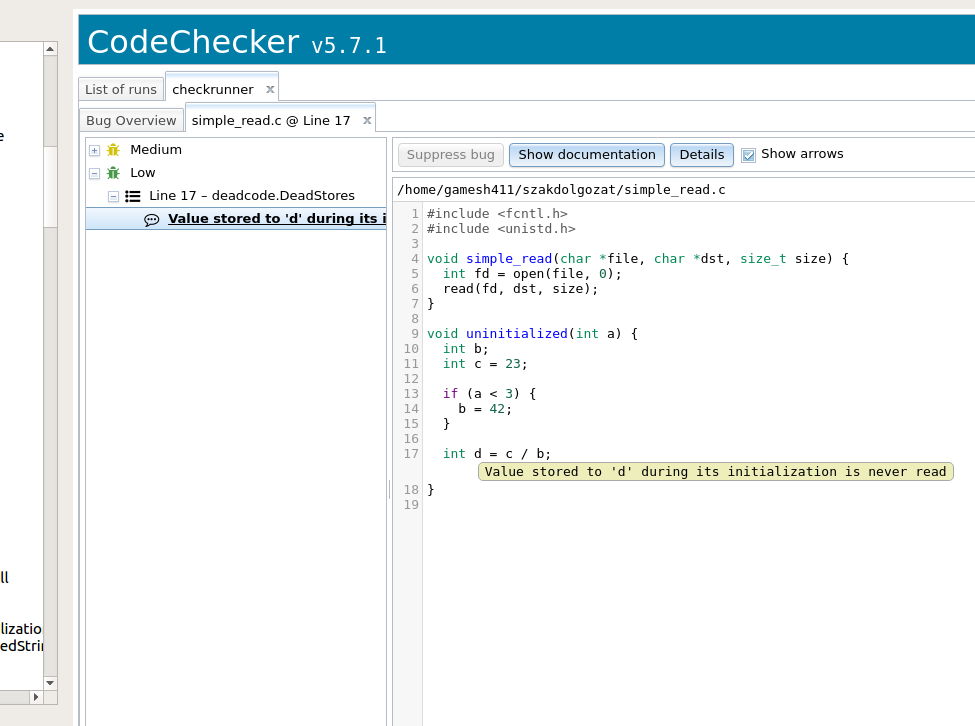
\includegraphics[scale=0.4]{ui_results_open.png}
\end{figure}

A program \texttt{File} menüjében egy \texttt{Open} és egy \texttt{Exit} művelet található. Az \texttt{Open} művelet ugyanazt a szerepet látja el, mint a build-könyvtárat kiválasztó gomb, de lehetőség van \texttt{Control-O} billentyűparanccsal az elérésére. Az \texttt{Exit} művelet értelemszerűen a kilépésre szolgál, billentyűparancsa a \texttt{Control-Q}. Emellett az ablakkezelő rendszer szokásos kicsinyítés és nagyítás, tálcára helyezés és befejezés műveleteit is használhatjuk.

\chapter{Fejlesztői dokumentáció}

\section{Grafikus felület}
A program felhasználói felülete a Qt \cite{qthomepage} eredetileg C++-ban írt rendszerét használja, mégis a CheckRunner végleges verziója Python nyelven került megvalósításra. A PyQt5 csomag gondoskodik a grafikus keretrendszer dinamikusan betölthető könyvtárainak elérhetővé tételéről. A modul írói elvégezték azokat a platformspecifikus illesztéseket, amelyek lehetővé teszik, hogy egy univerzális Python 3-as alkalmazás is ki tudja használni a Qt keretrendszer közel minden funkcióját.

A CheckRunner szoftveren való fejlesztésbe be lehet tehát kapcsolódni anélkül, hogy a felhasználói követelményeknél többet kellene teljesítenünk. A program alapvetően egy főablakból áll, amely modulárisan felhasznál három másik komponenst, hogy a CodeChecker háttérfolyamatokkal kommunikáljon. A program által megoldott problémák közül a háttérfolyamatokkal való kommunkáció volt a legérdekesebb. Előfordulnak egyszeri, gyorsan lefutó parancsok, hosszantartó folyamatok, melyekkel kommunikálni kell, és egy olyan folyamat is, amely maga is szülőprocessz-ként viselkedik, és amelynek megállítása nem vonja maga után a gyerekeinek a megállását sem. Ezen esetek a fejlesztés során szerzett tapasztalataim szerint mind előfordulnak.

\begin{figure}[h]
\caption{Alkalmazás-architektúra.}
\centering
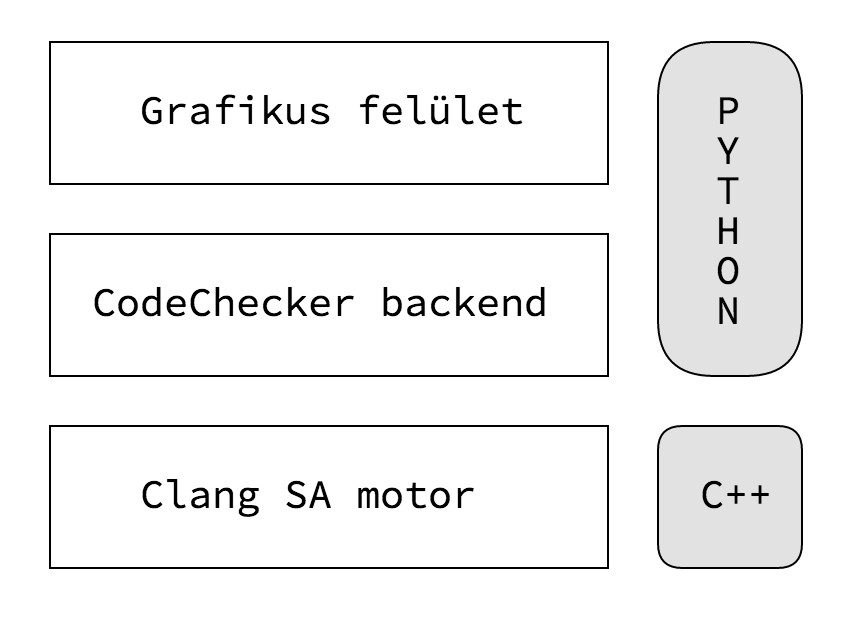
\includegraphics[scale=0.4]{architektura.png}
\end{figure}

A Qt rendszer egy eseményvezérelt működést támogató rendszer, ehhez a támogatáshoz szükség van bizonyos konvenciók betartására. Az eredeti C++-os rendszerben makrók segítségével köti össze a metaobjektum-fordító (MOC) az eseményvezérlést megvalósító signal és slot függvényeket. Ahhoz, hogy ez a rendszer működjön, a dinamikusan típusos Python esetében nincs ilyen előfeldolgozásra szükség, és megengedett jelzéskezelő függvények köre is jóval tágabb. Természetesen ennek futásidőben jelentkező következményei vannak, azonban a  program megalkotásakor fontosabb szempontnak tartottam, hogy széles körben legyen használható, egyszerű legyen a kihelyezés (deployment) és a fejlesztői környezet felállítása. A fejlesztés eredetileg C++ rendszerben kezdődött, azonban ezen szempontok miatt a végső megvalósítás mégis Python nyelven történt.

Meg kell említeni még, hogy a CodeChecker rendszer is Python nyelven íródott, és elképzelhető lenne a szorosabb integráció is. Ezt két szempont miatt vetettem el. Egyrészt a PyQt5 a Python nyelv hármas verzióját használja, a CodeChecker viszont a ketteset. A CodeChecker kódbázisának felületes áttekintése után megállapítható, hogy hozzáértő fejlesztők dolgoznak rajta, az esetleges integrációs törekvések nem ütköznének nagy problémába, azonban a CheckRunner alkalmazás megvalósításához nem volt erre szükség. A másik szempont az volt, hogy bemutassam a jól elkülönített komponensek flexibilisen összeállított rendszerét. A CheckRunner maga kis változtatásokkal képes lenne más, a CodeCheckerhez hasonlóan jól felszerelt futtatási környezetekkel együttműködni. Az ilyen megvalósítások manapság egyre terjedőben vannak, és a virtualizáció, illetve a konténer-technológia is hasonló megoldásokkal él.

A program forrásfájljait a mellékelt projektkönyvtáron belül a src mappában találhatjuk. A MainWindow felhasználja még a QtCreator segítségével megalkotott mainwindow.ui XML formátumú leírófájlt, illetve az ebből keletkezett Ui\_Main\_Window.py Python forrásfájlt. A PyQt5 pyuic5 parancssori alkalmazásával lehet a .ui fájlokat lefordítani. A használatához érdemes bekapcsolni a virtualenv környezetet, így bárhonnan elérhetjük a parancsot.

\begin{lstlisting}[caption={Virtuális környezet aktiválása.}
\label{lst:activatevirtualenv}]
source venv/bin/activate
\end{lstlisting}

\begin{lstlisting}[caption={UI fájlok lefordítása.}
\label{lst:pyuicusage}]
pyuic5 -o userinterface.py userinterface.ui
\end{lstlisting}

\begin{figure}[h]
\caption{Szerkezeti áttekintés.}
\centering
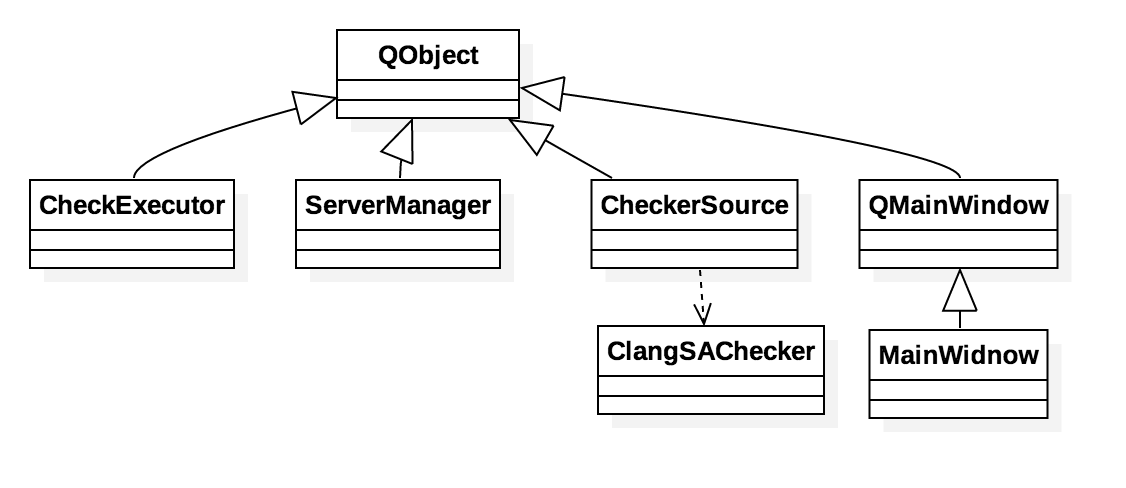
\includegraphics[scale=0.3]{UMLattekintes.png}
\end{figure}

A program MainWindow komponense felelős a felhasználói kezelőfelület aktuálisan tartásáért, illetve a felhasználó kéréseinek delegálásáért. A ServerManager komponens felel azért, hogy a program indításakor elinduljon a háttérben az analízis-eredmények fogadásáért és megjelenítéséért felelős CodeChecker folyamat, illetve erről visszajelzést adjon a MainWindow felé. A CheckerSource szolgáltatja az éppen aktuálisan használt Clang rendszerben elérhető ellenőrzéseket, és azt is, hogy alapértelmezetten be vannak-e kapcsolva. A CheckExecutor azért felel, hogy összegyűjtse a kívánt futtatás minden szükséges paraméterét, majd elindítsa a folyamatot, melynek keretében lefut az ellenőrzés, és a folyamat futásáról visszajelzést adjon a MainWindow felé.

Mindhárom alkomponens szignálokkal kommunikál a főablakkal, hogy az aszinkron működés miatt hatékonyan valósítsák meg az információ továbbítását. A ClangSAChecker egy adatosztály, mely egy Clang SA-beli checker-t szimbolizál. Eltárolja még, hogy a rendszerben alapértelmezetten be van-e kapcsolva ez a checker, illetve rendelkezik még egy statikus művelettel, mely segítségével a  CodeChecker rendszernek a checker-eket leíró szöveges reprezentációjából és képes példányokat előállítani, factory-ként működve ezáltal. A komponensek eseménykezelése legtöbb helyen igazából esemény továbbítás, a mélyebb szinten lévő folyamatok eseményeinek hatására váltanak ki saját event-eket, és ezekre válaszol a felhasználói felület, így a felhasználói felület osztályának szemszögéből a mögöttes folyamatok proxy-objektumaiként viselkednek. Ez a programtervezési minták körében egy igen elterjedt megoldás.

\begin{figure}[h]
\caption{Osztálydiagram.}
\centering
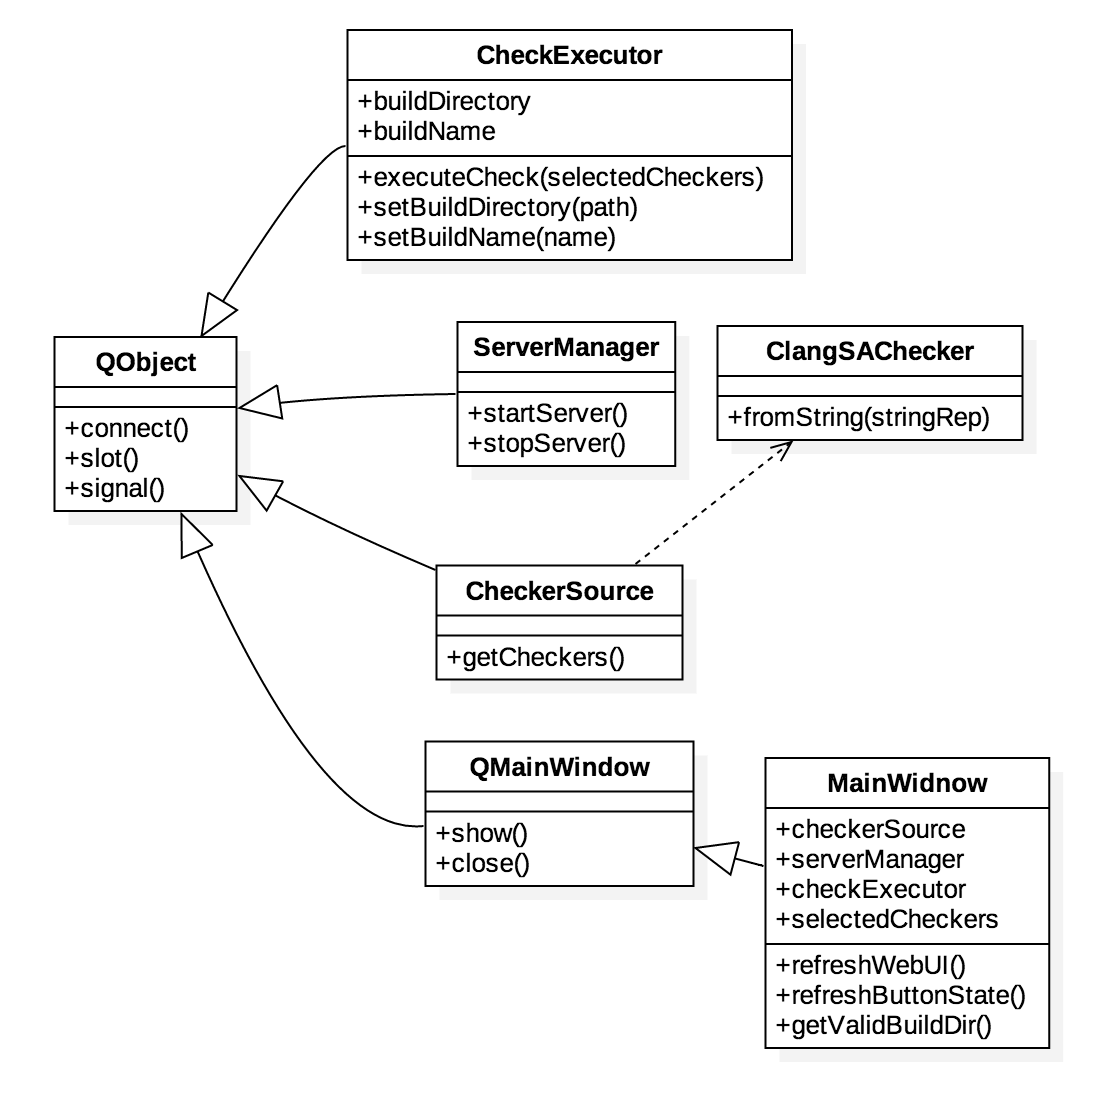
\includegraphics[scale=0.3]{osztalydiagram.png}
\end{figure}

A kiválasztott és nem kiválasztott checker-eket külön-külön listában tartjuk számon, mert alapvetően a CheckExecutor osztály executeCheck metódusának parancssori paraméterekkel kell felsorolnia, hogy mely checker-eket kívánja futtatni és melyeket kihagyni. A checker-ek leképezése a felhasználói felület kiválasztott elemeivé, illetve a fordított irányú konverzió a MainWindow osztályban zajlik le.

A CodeChecker hagyományos használatával ellentétben a CheckRunner nem egy parancs keretében tisztítja meg a build-könyvtára és építi újból a vizsgált projektet, hanem két egymást követő folyamat keretében. Ennek a QProcess osztály parancsértelmező képessége szab határt, nem tud beágyazott parancsokat kezelni. Emiatt a folyamatkezelés kissé bonyolultabb lesz az executeCheck metódusban.

A program a CodeChecker-rel való együttműködése során kihasználja  annak szolgáltatásait, egyrészt, hogy a checker-futtatás eredményét egy alapértelmezetten fájlalapú adatbázisban tárolja, másrészt, hogy ezzel az adatbázissal kommunikálva, webes felületen biztosít hozzáférést a CodeChecker az eredményekhez.

\begin{figure}[h]
\caption{Felhasználói esetek.}
\centering
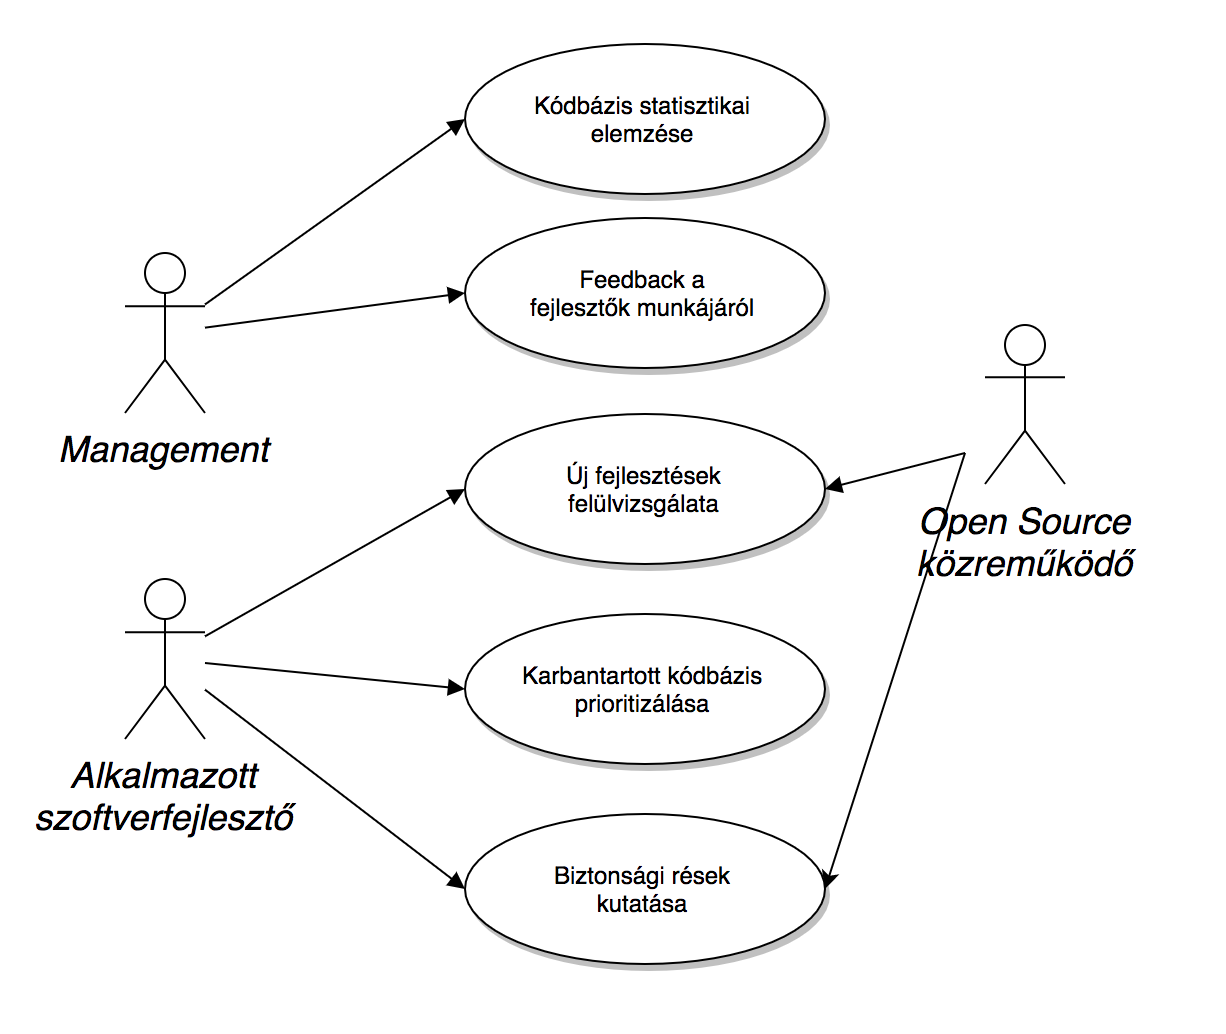
\includegraphics[scale=0.7]{felhasznaloi.png}
\end{figure}

\section{Checkerek}
Az általam megvalósított két checker a Clang SA részeként értelmezett modulok formájában létezik, ha ki szeretnénk próbálni, vagy mintájukra újabb checker-eket készíteni, akkor megtalálhatóak a mellékelt adathordozón. Mindkét checker esetében a forrásfájlt, és a teszteseteket tartalmazó fájlt mellékeltem, a checkers mappában, ezek alapján elvégezhető a 3.1 -es fejezetben már ismertetett folyamat, és készíthető egy olyan lefordított Clang példány, amely már rendelkezésünkre adja őket.

A statikus analízis folyamán a szimbolikus végrehajtást végző rendszer az AST alapján felépít egy CFG-t, majd ennek a gráfnak a segítségével modellezi az összes lehetséges futási útvonalat. Ezen lehetséges utak állomásai is egy gráfot képeznek, ezt a Clang SA \texttt{Exploded Graph}-nak hívja, és egy \texttt{ProgramPoint} és egy \texttt{ProgramState} típusú objektummal reprezentálja egy csúcsát. A \texttt{ProgramPoint} megmondja, hogy a CFG-n belül hol jár a program, a \texttt{ProgramState} pedig a program és az éppen futó ellenőrzés közös állapotát írja le. A \texttt{ProgramState} három fő komponenssel bír:

\begin{itemize}
\item környezeti információ, vagyis hogy az aktuális futási helyzetben milyen megfeleltetés érvényes a programkódbeli kifejezések és szimbolikus értékük között
\item memória információ, vagyis hogy a futás ezen pontján milyen feltételezésekkel élhetünk a program memóriáját illetően
\item általános adatok, az ellenőrzés során a checker-ek által összegyűjtött adatok jelenlegi értéke
\end{itemize}

A checker-ek úgy működnek, hogy amikor a Clang SA szimbolikus végrehajtást végez, akkor minden programkódbeli kifejezés, illetve utasítás során annak típusától függően futtatja a megfelelő checker-t vagy checker-eket. Ez a megvalósítás a megfigyelő (observer) programozási minta egy jó példája, a checker megfigyelőként feliratkozik azokra az utasítástípusokra, amelyek számára érdekesek, és Clang SA elemzési folyamatai során a feliratkozott checker-eket értesíti, hogy bekövetkezett a megfelelő utasítás feldolgozásának eseménye.

Amikor egy checker-t megvalósítunk, az első fontos döntés, hogy milyen eseményekre, vagyis milyen típusú kifejezések feldolgozására iratkozunk fel. Ennek a hátterében az áll, egy adott probléma esetében ki kell dolgoznunk a probléma megoldását, de a statikus analízis nyelvén, vagyis egy olyan algoritmust kell találnunk, amely tudja, hogy milyen milyen kifejezések érdekesek a számára, és ezekre hogyan reagáljon.

A OStreamFormatChecker célkitűzése az volt, hogy adjon figyelmeztető üzenetet abban az esetben, ha valaki átállított egy formázási opciót egy kimeneti stream objektumon, és utána elfelejtette visszaállítani azt, ha már nem használja. Ebben az esetben több probléma is felmerül. A kód írója bármikor átállíthatja ezeket a formátumjelzőket olyan céllal, mert neki nem tetszik az alapértelmezett beállítás és végig máshogy szeretné használni a kimenetet. Emellett előfordulhat, hogy valaki csak egy környezetben szeretné máshogy használni a stream objektumot. Az tehát, hogy mikor felejtett el valaki valamilyen beállítást visszaállítani (ha egyátalán vissza akarta valaha), nem triviális kérdés. Mégis vannak olyan esetek, amikor jobbnak látjuk, hogy figyelmeztetést kapunk, mintsem akkor lepődjünk meg, vagy esetleg egy másik komponens, amely utánunk használja a kimenetet, hogy nem a szokványos formázással jelennek meg az adatok.

Az OStreamFormatChecker esetében a következő formában fogalmaztam meg az eredeti problémát a programozási nyelvek konstrukciói alapján: Adjon a checker hibaüzenetet, ha egy függvényhívás végére érünk, és ennek a függvényhívásnak blokkjában (vagyis lexikális környezetében) volt olyan módosítás egy kimeneti streamben, ami nem lett visszaállítva az alaphelyzetbe. Kivételt képez az az eset, ha egy stream objektumtól lekérdezték a formátumait jelző állapotbiteket. Ilyenkor azt feltételezzük, hogy aki lekérte ezeket az majd vissza is fogja állítani az eredeti állapotot (más praktikus célja nem nagyon létezik a formátum-flagek lekérésének). Ez már az eredeti problémát elég jól közelítő modell.

Az OStreamFormatChecker tehát megvalósítását tekintve feliratkozik az \texttt{EndFunction} eseményre, itt lehetséges felfedezni az állapot-visszaállítás hiányát, illetve feliratkozik még a \texttt{PreCall} és \texttt{EvalCall} eseményekre, mert ezek tudják megváltoztatni a stream állapotát. Egy stream állapota ráadásul több úton is változhat. Van, hogy az objektumon direkt módon meghívunk egy tagfüggvényt, de lehetőségünk van manipulátorok használatára is.

\begin{lstlisting}[caption={OStream objektumok formázásának megváltoztatása.}
\label{lst:activatevirtualenv}]
double var = 117.123456789123456;
std::cout.setprecision(12);
std::cout << var;
// prints 117.123456789123
std::cout << std::setprecision(3) << var;
// prints 117.123
\end{lstlisting}

A megvalósítás során felhasználjuk a Clang SA által a checker-eknek biztosított tárolási lehetőséget egy asszociatív (map) jellegű tároló formájában. Minden stream-et a memóriában elfoglalt helye alapján azonosítunk, és ehhez, mint kulcshoz rendeljük a saját magunk által számon tartott formázási állapotok struktúráját, illetve hogy eredetileg melyik függvényben történt az első változtatás. Így a szimbolikus végrehajtás során minden alkalommal, amikor egy egyező memóriaterületű stream objektumon módosítást tapasztalunk, akkor feljegyezzük. Az \texttt{EndFunction} eseményre ezután már könnyű reagálni. Csak meg kell nézni, milyen streamek állapotait tartjuk számon azok közül, amelyiknél a bejegyzett első módosítás környezete éppen az a függvény, amiből kilépünk. Ha az állapotok közül ilyenkor egy is eltér az alapértelmezettől, akkor hibaüzenetet adunk. Itt kezeljük még a kivételes esetet is, amikor volt \texttt{.flags()} hívás az objektumon. Ilyen esetben nem adunk hibát bármilyen is legyen a számon tartott stream.

\begin{figure}[h]
\caption{A két checker egyszerűsített osztálydiagramja.}
\centering
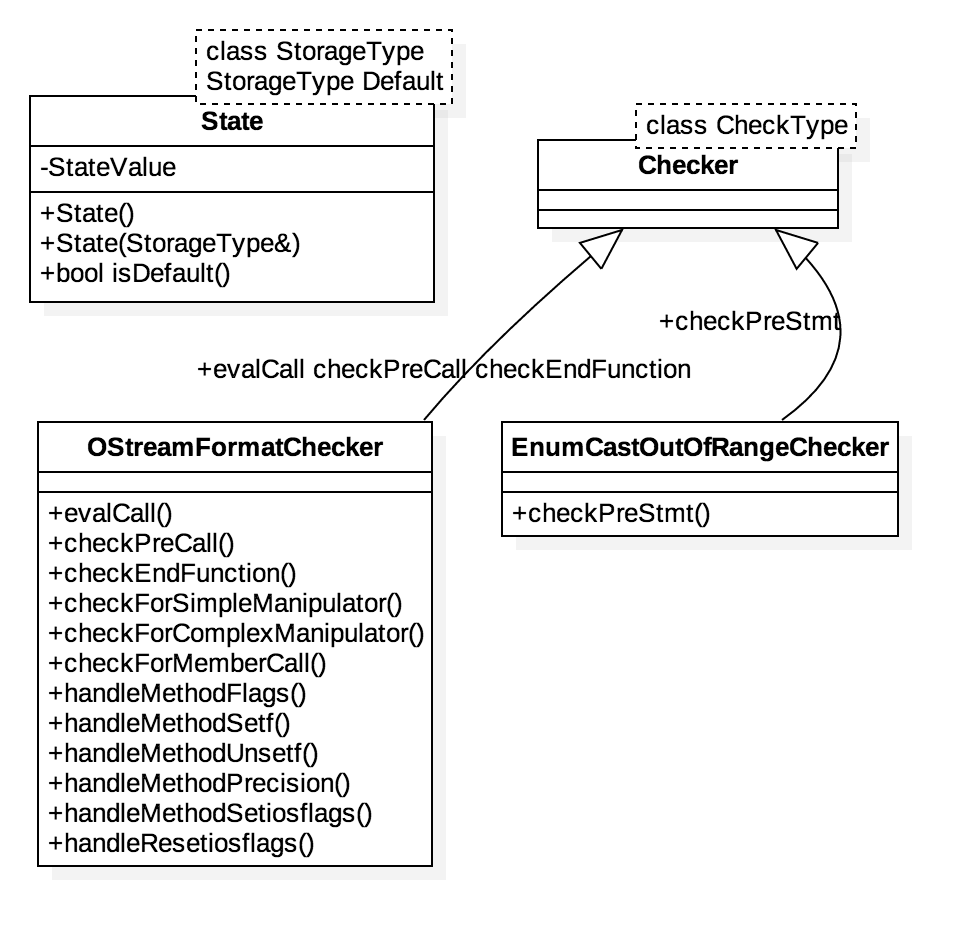
\includegraphics[scale=0.4]{checkers.png}
\end{figure}

Az EnumCastOutOfRange checker egyszerűbb felépítésű. Itt a feladat az volt, hogy akkor adjunk hibát, hogy ha egy olyan típuskikényszerítés (cast) történik, melynek operandusa egy egész értéktípusba tartozó érték, és a paramétere, vagyis az a típus, amibe kényszerítjük egy olyan enumeráció típus, amely típus definíciójából kiderül, hogy nem is képes reprezentálni az operandust.

\begin{lstlisting}[caption={Enumeráció hibás cast-olása.}
\label{lst:activatevirtualenv}]
enum GraphNode {
	WHITE = 0,
	GRAY,
	BLACK
};
GrapNode startNode = static_cast<GraphNode>(5);
//startNode's value is undefined
\end{lstlisting}

Ilyen esetben ha nem képes az enumerációs típus tárolni az értéket, akkor cast eredménye nem definiált. Ahhoz, hogy egy enumerációs típus használni tudjunk szükség van a definíciójára a használat pontján, így azt a stratégiát választottam, hogy iratkozzon fel a checker a \texttt{PreStmt}, vagyis pre-statement, egy utasítás végrehajtása előtti eseményre. Abban az esetben, ha ez az utasítás egy cast-ot jelent (ez lehet C-stílusú, vagy lehet C++-os static\_cast), és ráadásul a céltípus enumerációs jellegű, akkor megvizsgálom, hogy ez a művelet a probléma kitűzése szerint valid lehet-e.

Ehhez egyik oldalról szükség van az enumeráció definíciójára, ez rendelkezésre is áll. A definíció egyszerűen megtalálható, és ha mint AST egy szelete hozzáfértünk, akkor meg is tudjuk belőle a lehetséges értékeket. Másik oldalról szükséges számunkra az érték, amit cast-olunk. Ez sokszor nehezebb, és a checker kihasználja, hogy szimbolikus értékekkel történik a végrehajtás. A szimbolikus értékek valójában a valós futás során ténylegesen létező értékeket szimbolizálják megkötések (constraint-ek) formájában. Még ha nem is ismert az operandus konkrét értéke, a Clang SA által vezetett megszorításlisták segítségével ellenőrizhetjük, hogy létezik-e olyan eset, hogy az operandus valóban megfelelő értékkel bír. Akkor adunk hibát, ha nem létezik ilyen eset, hiszen egyik célunk, hogy ne produkáljunk hamis pozitív jelzéseket, ezért konzervatív módon járunk el.


\chapter{Tesztek}

Mindkét checker-em rendelkezik automatizált unit-tesztekkel. Az OStreamFormatChecker tesztelése során külön nehézséget jelentett, hogy az egyik legvalószínűbb tesztelési célpont a sztenderd kimenetet szimbolizáló \texttt{std::cout}, ez pedig megvalósítását tekintve úgy működik a legtöbb sztenderd nyelvi könyvtár (STL) megvalósításban, hogy az iostream header tartalmaz egy statikus tagot, amely tárolja a globális \texttt{std::cout} stream objektumot. Emiatt a viselkedése miatt az egész \emph{LLVM} kódbázisból ki van tiltva az iostream header használata. Ahhoz, hogy tesztelni tudjam a checkert létre kellett hozni az STL-es output rendszer a vázát, amely alapján ha implementáció nélkül is, de szintaktikailag helyesen lehet hivatkozni a tesztesetek közben az \texttt{std::cout} objektumra, és a rá értelmezett műveletekre. Ez a mock-megvalósítás maga legalább annyi időt vesz igénybe mint a tesztesetek megírása, viszont sokat segíthet másoknak is akik hasonló funkcionalitás tesztelésébe fognak.

Az OstreamFormatChecker tíz automatizált tesztesete lefedi a tesztelni kívánt működés nagyrészét. Van benne egyszeri módosítás, több módosítás egymásutánja, az értékek visszaállítása, illetve ennek elmulasztása, és vannak benne olyan esetek, amikor a szimbolikus végrehajtónak a megszorítások alapján kell kitalálnia, hogy tényleg történt-e módosítás vagy nem. Az EnumCastOutOfRange tizenhat tesztesettel rendelkezik C-stílusú és C++ cast-olásokra, illetve megadott háttértípussal rendelkező és hagyományos, C-beli globálisan értelmezett és C++11-es láthatósági körrel rendelkező enumerációkra egyaránt.

A manuális futás során nagyobb kódbázisokon is lefuttattam az ellenőrzőt, és a futás minden esetben problémamentes volt. A keretrendszer tesztelésre került több open-source könyvtáron, és a program saját kódján is. Az Ericssonnál végzett munkám során lehetőségem nyílt sok nagy méretű, nyílt forráskódú projekten látni a Clang Static Analyzer eredményeit, többek között az OpenSSL, ffmpeg, tmux, memcached, nginx és vim könyvtárakon, és ezek mind működnek a CheckRunner szoftveren keresztüli használat során is.

A saját checker-eim manuális teszteredményei közül két példát mutatok be a Boost \cite{boosthomepage} könyvtárban, amikor az OStreamFormatChecker hibát jelzett. Mindkettő a \texttt{Boost 1.63.0}-ás verziójában fordult elő. A Boost projekt moduljai között több olyan van, ami nem köthető build-rendszerhez. Az ilyen könyvtárak esetében nem egy különálló fájlban van az implementáció, hanem csak header-állományokból állnak. Ebben fájlban együtt él a deklaráció és a definíció, és jellemzően hpp kiterjesztéssel rendelkezik. A Clang SA parancssori futattását alkalmaztam az egyes hpp állományokra.

\begin{lstlisting}[basicstyle=\tiny,caption={Boost print hiba.}
\label{lst:boostprintmacroerror}]
static unsigned int indent = 4;
static unsigned int width = 40;

void print_macro(const char* name, const char* value)
 {
    // if name == value+1 then then macro is not defined,
    // in which case we don't print anything:
    if(0 != strcmp(name, value+1))
    {
       for(unsigned i = 0; i < indent; ++i) std::cout.put(' ');
       std::cout << std::setw(width);
       cout.setf(istream::left, istream::adjustfield);
       std::cout << name;
       if(value[1])
       {
          // macro has a value:
          std::cout << value << "\n";
       }
       else
       {
          // macro is defined but has no value:
          std::cout << " [no value]\n";
       }
    }
 }
\end{lstlisting}

\begin{minipage}{\linewidth}
\begin{lstlisting}[basicstyle=\tiny,caption={Boost exception hiba.}
\label{lst:boostexecptionerror}]
namespace boost {

//  progress_timer  ----------------------------------------------------------//

//  A progress_timer behaves like a timer except that the destructor displays
//  an elapsed time message at an appropriate place in an appropriate form.

class progress_timer : public timer, private noncopyable
{

 public:
  explicit progress_timer( std::ostream & os = std::cout )
     // os is hint; implementation may ignore, particularly in embedded systems
     : timer(), noncopyable(), m_os(os) {}
  ~progress_timer()
  {
  //  A) Throwing an exception from a destructor is a Bad Thing.
  //  B) The progress_timer destructor does output which may throw.
  //  C) A progress_timer is usually not critical to the application.
  //  Therefore, wrap the I/O in a try block, catch and ignore all exceptions.
    try
    {
      // use istream instead of ios_base to workaround GNU problem (Greg Chicares)
      std::istream::fmtflags old_flags = m_os.setf( std::istream::fixed,
                                                   std::istream::floatfield );
      std::streamsize old_prec = m_os.precision( 2 );
      m_os << elapsed() << " s\n" // "s" is System International d'Unites std
                        << std::endl;
      m_os.flags( old_flags );
      m_os.precision( old_prec );
    }

    catch (...) {} // eat any exceptions
  } // ~progress_timer

 private:
  std::ostream & m_os;
}; 
\end{lstlisting}
\end{minipage}

Ennek a hibának az az érdekessége, hogy a kód írója külön figyelmet fordított a formázási flag-ek visszaállítására, de ha kivétel lép fel, akkor mégsem garantált az alapértelmezett állapot visszaállítása.

\chapter{Összefoglalás}
Szakdolgozatomban ismertettem a modern szoftverfejlesztés eszköztárának fontosabb elemeit. Összehasonlításra került a statikus és a dinamikus kódelemzési stratégia, külön hangsúlyt fektetve a statikus elemzés jellegzetességeire. Emellett több példán keresztül bemutatásra került az eszköztár, illetve a modellezési módszerek, amelyek ezt lehetővé teszik. Kiterjesztést nyert a \emph{Clang} keretrendszer is, több hibát képes felismerni a két checker-nek köszönhetően, mint azelőtt. Bemutattam az \emph{LLVM} és a \emph{Clang} eszköz felhasználási lehetőségeit egy praktikus program keretében, mely statikus elemzéshez kapcsolódó eszközöket fogott össze egy grafikus felületbe.

A program számos továbbfejlesztési lehetőséggel rendelkezik. A \emph{CodeChecker} rendszerrel való hatékonyabb integráció lehetséges anélkül, hogy feláldozzuk a moduláris felépítést. A \emph{CodeChecker} szoftvernek modern elvárásokkal összhangban zajló virtualizálása jelenleg fejlesztés alatt áll, egy \emph{Docker} konténer segítségével lehetőség lesz akár felhőalapú futtatására is. A CheckRunner szoftver illeszthető lehet az ilyen jellegű használathoz.

A statikus forráselemzés a modern szoftverfejlesztés szerves részévé vált, a kódminőség javítása érdekében érdemes automatizált futtatóeszközök által élni a lehetőségeivel. Sok hiba felfedezésre kerül, amelyeket lehetetlen, vagy igen körülményes lenne a futásidejű elemzések segítségével megtalálni. A példaprogram szerkezetileg jól illusztrálja, amit már a \emph{Clang} működése során, és a kapcsolódó scan-build-py, és \emph{CodeChecker} programok működése során is láttunk, miszerint több lazán kapcsolódó komponens segítségével nagyon flexibilis szoftveres megoldásokhoz juthatunk.

\begin{thebibliography}{xx}

\bibitem{umlverification} Makan Pourzandi {\em Formal Verification and Validation of UML
2.0 Sequence Diagrams using Source and
Destination of Messages}.  2009 https://doi.org/10.1016/j.entcs.2009.09.064 2017.04.28.

\bibitem{interpretedtransforms} Bücker H.M., Petera M., Vehreschild A. (2008) {\em Code Optimization Techniques in Source Transformations for Interpreted Languages.} In: Bischof C.H., Bücker H.M., Hovland P., Naumann U., Utke J. (eds) Advances in Automatic Differentiation. Lecture Notes in Computational Science and Engineering, vol 64. Springer, Berlin, Heidelberg

\bibitem{transpilation} Javascript nyelvi transzformációk. https://thenewstack.io/javascript-transpilers-need-know/ 2017.04.28

\bibitem{chaosmonkey} Chaos Monkey. https://insights.sei.cmu.edu/devops/2015/04/devops-case-study-netflix-and-the-chaos-monkey.html 2017.04.28

\bibitem{llvmhomepage} LLVM honlap. http://llvm.org/ 2017.04.29

\bibitem{llvmarchitecture} LLVM könyv http://www.aosabook.org/en/llvm.html 2017.04.29

\bibitem{simplecompilerimage} Egyszerűsített fordítómodell. http://www.aosabook.org/images/llvm/SimpleCompiler.png 2017.04.29

\bibitem{lattnerhomepage} Chris Lattner weboldala. http://nondot.org/~sabre/ 2017.04.29

\bibitem{clangusermanual} Clang hivatalos felhasználói dokumentáció. https://clang.llvm.org/docs/UsersManual.html 2017.05.03

\bibitem{clangdriverinternals} Clang driver leírás. https://clang.llvm.org/docs/DriverInternals.html 2017.05.03

\bibitem{clangtoolchain} Clang fordítóeszközök. https://clang.llvm.org/docs/Toolchain.html 2017.05.03

\bibitem{clangdriverimage} Clang driver szerkezet. https://clang.llvm.org/docs/\_images/DriverArchitecture.png 2017.05.03

\bibitem{clangsahomepage} Clang SA weboldal. http://clang-analyzer.llvm.org/ 2017.05.04

\bibitem{clangsapathsensitiveimage} Clang SA XCode integráció. http://clang-analyzer.llvm.org/images/analyzer\_xcode.png 2017.05.04

\bibitem{clangsaimage} Clang SA HTML nézet. http://clang-analyzer.llvm.org/images/analyzer\_html.png 2017.05.04

\bibitem{libclangdocs} LibClang dokumentáció. https://clang.llvm.org/doxygen/group\_\_CINDEX.html 2017.05.05

\bibitem{clangtooling} Clang könyvtárak dokumentáció. https://clang.llvm.org/docs/Tooling.html 2017.05.05

\bibitem{codecheckergit} CodeChecker kódbázis. https://github.com/Ericsson/codechecker 2017.05.05

\bibitem{getllvmpage} LLVM felhasználói dokumentáció. http://llvm.org/docs/GettingStarted.html 2017.05.05

\bibitem{checkerdevmanual} Clang SA checker dokumentáció. http://clang-analyzer.llvm.org/checker\_dev\_manual.html 2017.05.05

\bibitem{securecodingint50} INT50-CPP specifikáció. https://www.securecoding.cert.org/confluence/display/cplusplus/INT50-CPP.+Do+not+cast+to+an+out-of-range+enumeration+value 2017.05.06

\bibitem{codecheckerslide} CodeChecker szerkezet. https://www.slideshare.net/GyorgyOrban/static-analysis-of-c-programs 2017.05.08

\bibitem{qthomepage} Qt grafikus keretrendszer honlapja. https://www.qt.io/ 2017.05.12

\bibitem{boosthomepage} Boost C++ könyvtár honlapja. http://www.boost.org/ 2017.05.13

\bibitem{dockerhomepage} Docker weboldal. https://www.docker.com/ 2017.05.12

\end{thebibliography}
\end{document}
